In this section we present our results obtained by the full frequency dependent fRG. All the results are presented in units of the nearest-neighbor hopping $t=1$. Unless specified otherwise, the next-nearest-neighbor hopping is $t'=-0.32t$, the interaction strength $U=4t$, and the temperature $T=0.08t$.

We have implemented numerically the flow equations reported in the appendix. 
To take into account the distinct momentum dependences of the self-energy and the vertex, we have defined two different patching schemes of the respective Brillouin zones. 
%The $\phi$-functions depend on a momentum transfer.  
%For the filling and nearest neighbors hopping that we want to describe, the momentum vectors of the most relevant process are $\mathbf{Q}=(0,0)$, important for superconductivity (in the pairing channel) and ferromagnetism (in the magnetic channel); $\mathbf{Q}=(\pi,\pi)$ and its vicinity, relevant for antiferromagnetism and incommensurate antiferromagnetism; the momentum transfer $2k_F$, as defined in Ref.~\onlinecite{Holder2014}, associated to the onset of charge- and spin-density wave instabilities. 
Similarly to what is done in Ref.~\onlinecite{Husemann2009}, the vertex patching describes more accurately the corners around $(0,0)$ and $(\pi,\pi)$, where we expect the instability vectors.
For the self-energy, the most relevant physics happens in the vicinity of the Fermi surface.
Therefore we concentrate the patches along the Fermi surface and in its immediate vicinity (see Figs. \ref{fig:selffermi0975} and \ref{fig:selffermi0600}), with more points close to the \textit{antinodal} region near $(\pi,0)$, relevant for antiferromagnetism.
In the calculations presented in the following we have used $29$ patches for the vertex and $44$ for the self-energy.

For the implementation of the frequency dependence we found it convenient to rewrite $\mathcal{S}$, $\mathcal{D}$, $\mathcal{C}$ and $\mathcal{M}$ as functions of three bosonic frequencies. 
For each frequency argument we restricted ourselves to at least $40$ positive and $40$ negative Matsubara frequencies. Beyond these frequencies we have used the asymptotic values. 
%The number of Matsubara frequencies that can be taken into account sets the lowest temperature reachable by the calculation.

\subsection{Analysis of instabilities}

By means of the fRG one can perform an instability analysis of the system: 
for some value of the flow parameter $\Lambda$ one of the channels shows a divergence. 
The value $\Lambda_{\mathrm{c}} $ for which this happens is called \textit{critical scale}, and from the diverging channel one can infer the leading instability of the system. 
%
\begin{figure}
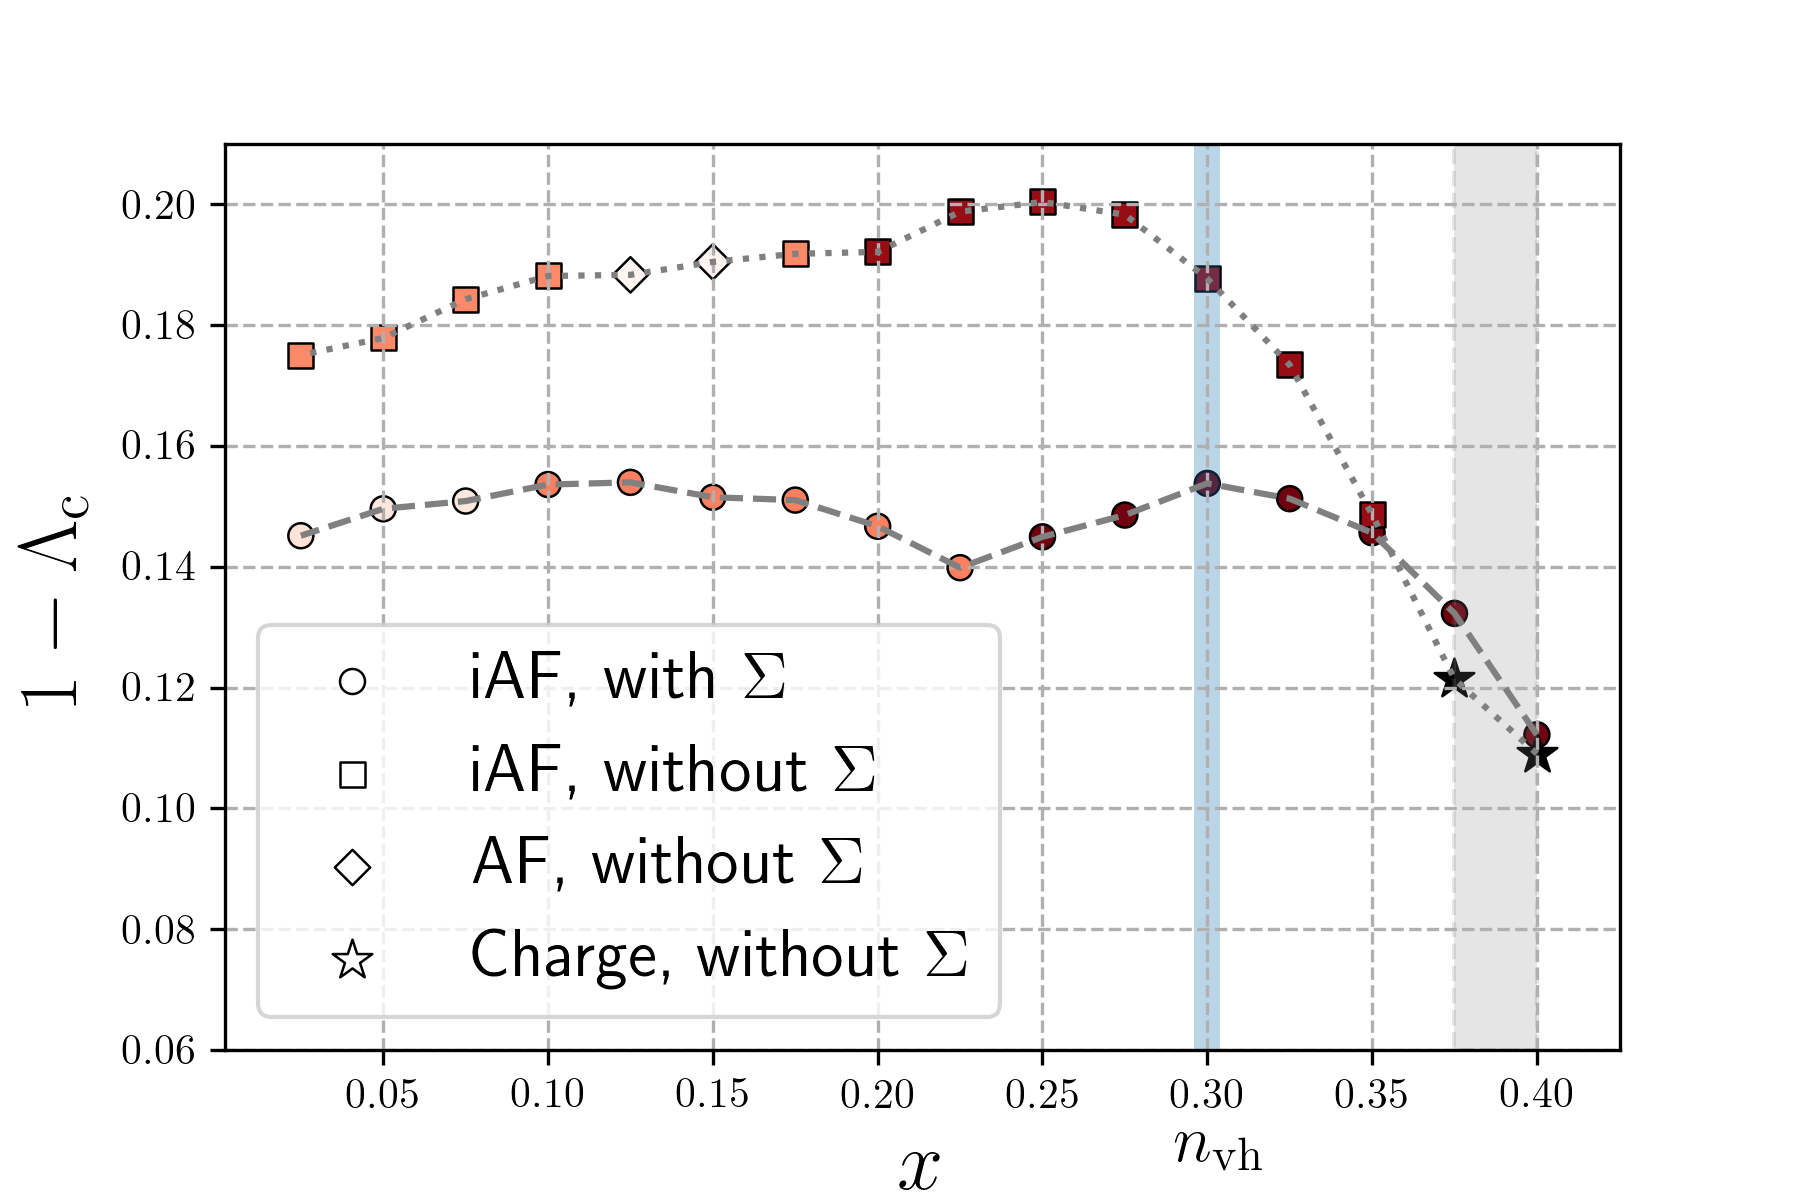
\includegraphics[width=0.5\textwidth]{images/phasediag.png}
\caption{Critical scale $1-\Lambda_{\mathrm{c}}$ as a function of doping $x=1-n$, for $T = 0.08t$, $t'=-0.32t$ and $U=4t$. 
Square symbols and circles refer to incommensurate antiferromagnetism (iAF) without and with self-energy feedback, respectively.
The black stars refer to a divergence in the charge channel at $\mathbf{Q} = (0,0)$.
The color of squares and circles encodes the distance of the incommensurate magnetic $\mathbf{Q}$-vector from $(\pi,\pi)$: darker color corresponds to a larger distance. The darkest color corresponds to $\delta=1.13$. 
The vertical light blue line marks van Hove filling.}  
\label{fig:criscale} 
\end{figure}
%
In Fig.~\ref{fig:criscale} we show the critical scale $1-\Lambda_{\mathrm{c}}$ as a function of the doping $x=1-n$ with and without self-energy feedback.
%We show our result in terms of $1-\Lambda$, which vanishes at the end of the flow. 
For the physical interpretation of $\Lambda_c$ in the interaction flow, we refer to the rescaled interaction\cite{Honerkamp2004} $\tilde U ^\Lambda$ discussed in Sec.~\ref{sec:cutoff}.  

We defined the critical scale as the flow parameter for which the value of the largest channel exceeds $200t$. We checked that these results are also consistent with a stability analysis based on the susceptibilities.        

A divergence of the vertex at finite temperature is associated with spontaneous symmetry breaking, in violation of the Mermin-Wagner theorem.\cite{Mermin1966}
This is a consequence of the truncation of the flow equations.
%since in our truncation-scheme we do not include the bosonic-fluctuations of the order parameter\cite{Baier2004}, essetial to obtain a vanishing critical temperature. 
Instead, we should interprete the finite temperature vertex divergence as the signal of the appearance of strong bosonic fluctuations that cannot be treated within the approximation-scheme we are using.\cite{Salmhofer2001} 
Even though in our framework the flow cannot be continued beyond the critical scale, from the analysis of vertex and self-energy we can identify the relevant effective interactions of the system.

%In the specific case of the interaction cutoff we can interprete the rescaled interaction $\tilde U^{\Lambda_\mathrm{c}}$ as the critical interaction at a given temperature.
For the parameter sets shown in Fig.~\ref{fig:criscale}, and without self-energy feedback, there are two possible instabilities. 
For doping smaller than $0.35$ the leading fluctations of the system are either commensurate or incommensurate antiferromagnetic.
The incommensurability $\delta$ is defined through $\mathbf{Q}=(\pi,\pi-\delta)$, the momentum where the magnetic channel $\mathcal{M}^\Lambda$ has its maximum. 
The region of commensurate antiferromagnetism for $0.125\le x \le 0.150$ has to be attributed to the presence of a large plateau around $(\pi,\pi)$ in the bare bubble. Correspondingly, the commensurate antiferromagnetic instablility is almost degenerate with an incommensurate one.
%
\begin{figure}
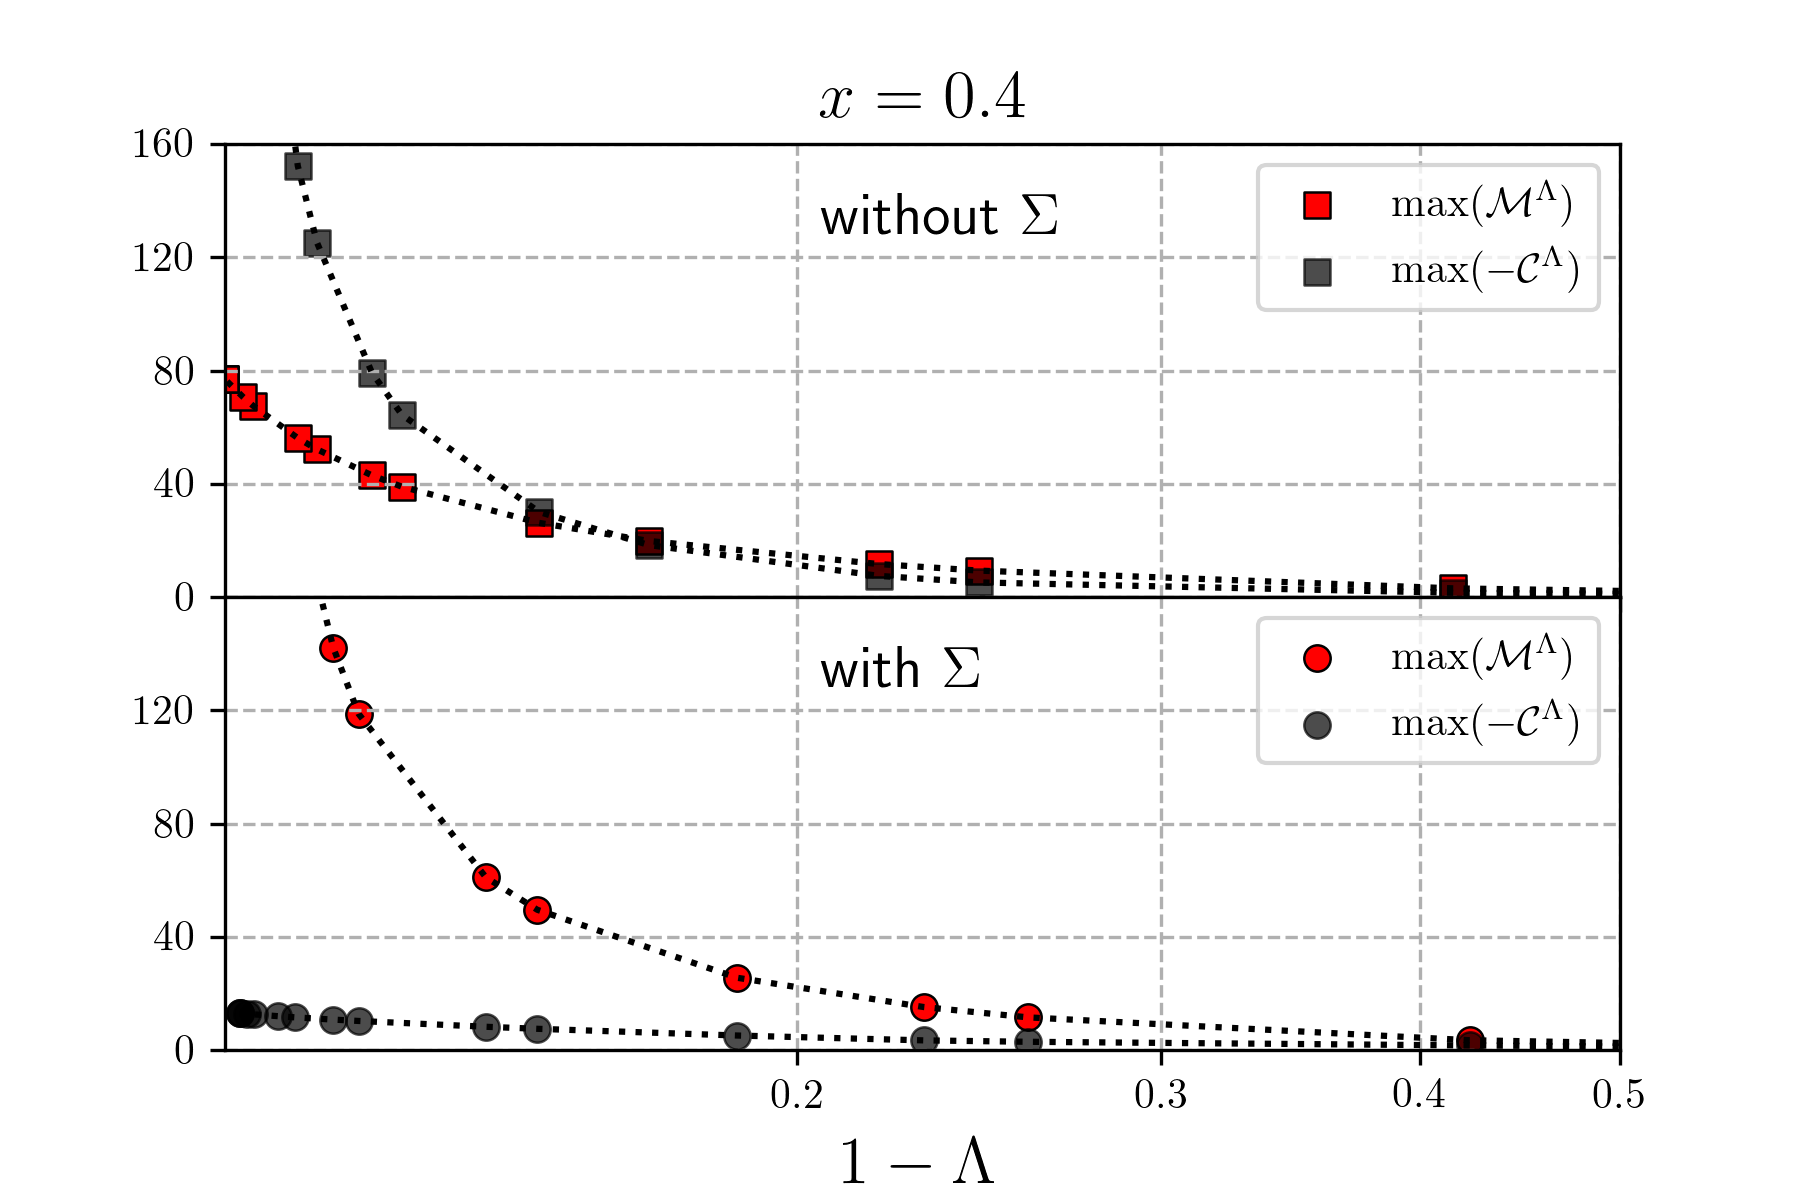
\includegraphics[width=0.50\textwidth]{images/chargeproblem_MC_vs_Lambda_fix_occ.png}
\caption{Flow of the maximal values of the charge ($\mathcal{C}$) and magnetic ($\mathcal{M}$) channels as functions of $1-\Lambda$, for  $x=0.4$, $t'=-0.32$, $U=4t$ and $T=0.08t$.  Top: without self-energy feedback; bottom: with self-energy feedback. }
\label{fig:chargeproblem}
\end{figure}
%

The most striking feature in Fig.~\ref{fig:criscale} is the presence of a divergence in the charge channel $\mathcal{C}^\Lambda$ at $\mathbf{Q}=(0,0)$ for the largest values of doping, marked by black stars. 
This feature was already observed in a fRG calculation with a simplified frequency parametrization by Husemann \textit{et al.} in Ref.~\onlinecite{Husemann2009}, and named \textit{scattering instability}. 
The charge channel $\mathcal{C}^\Lambda$ diverges for finite frequency transfer $\Omega=2\pi T$, which does not allow for a natural interpretation in terms of a physical instability. 
The frequency structure of the charge channel $\mathcal{C}^\Lambda$ together with its origin will be discussed further in paragraph \ref{sec:per_ladder}.

\begin{figure}
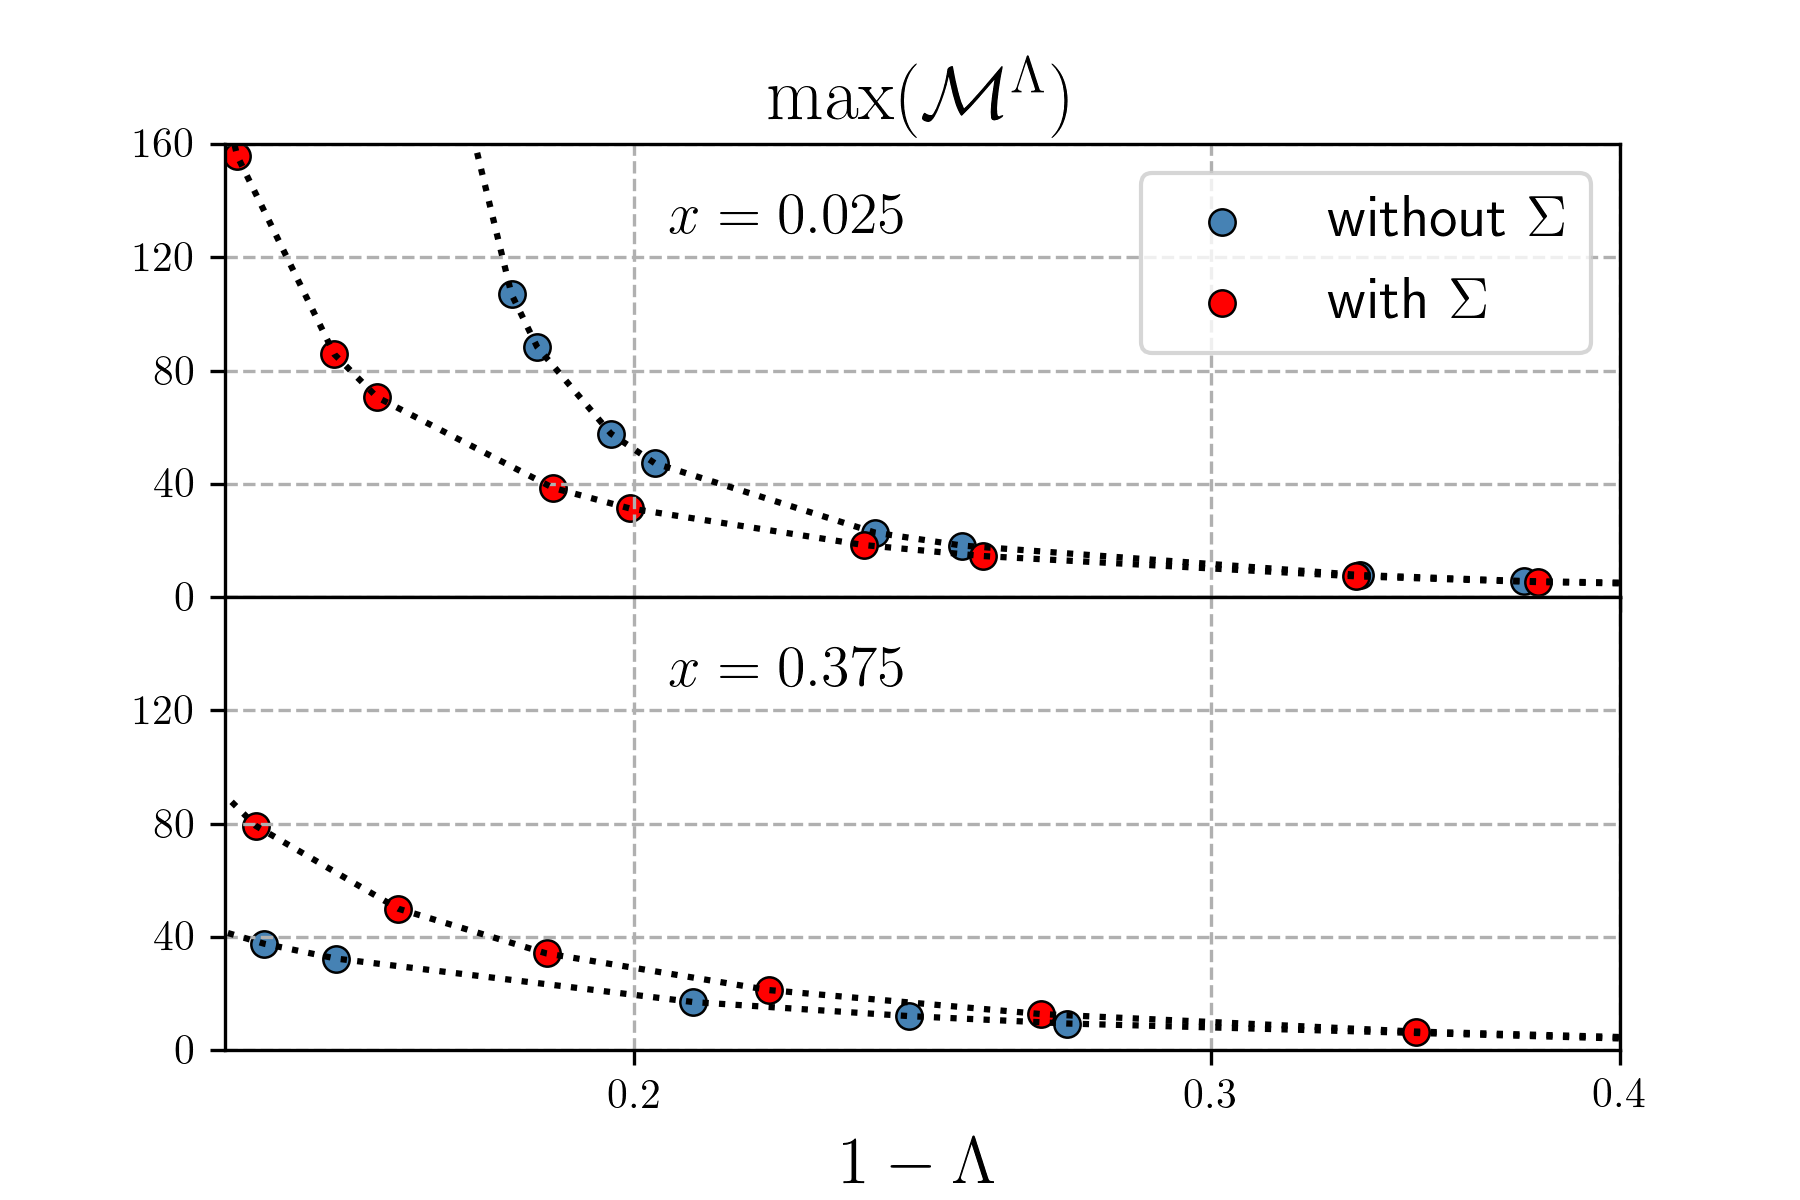
\includegraphics[width=0.50\textwidth]{images/chargeproblem_M_vs_Lambda_diff_occ.png}
\caption{Flow of the maximal values of the  magnetic ($\mathcal{M}$) channel as functions of $1-\Lambda$, for  $x=0.025$ (top) and $x=0.375$ (bottom). The other parameters are $t'=-0.32$, $U=4t$ and $T=0.08t$. Red symbols: with self-energy feedback; blue symbols: without self-energy feedback. }
\label{fig:selfeffect}
\end{figure}

The self-energy feedback has three effects. First, it decreases $1-\Lambda_c$.
Second, the incommensurability vector is affected, the region of commensurate antiferromagnetism disappears, and one can observe a more regular trend of increasing $\delta$ with $x$.
Third, the divergence in the charge channel is completely suppressed, and the leading instability in the doping region $0.375\le x \le 0.4$ remains incommensurate antiferromagnetic. 
This can be also seen from Fig.~\ref{fig:chargeproblem}, where we compare the flow of the maximum (of the absolute value) of magnetic and charge channels with and without the self-energy feedback for doping $x=0.4$.
Without self-energy feedback, the charge channel reaches large and negative values.
The presence of such a large (and negative) charge channel inhibits the magnetic channel.    
The effect of the self-energy in the flow is evident: the charge channel is strongly damped.  
At the same time the magnetic channel is enhanced.

This is confirmed by Fig.~\ref{fig:selfeffect}, where we show the maximum of $\mathcal{M}$ with and without self-energy feedback for $x=0.025$ (top) and $x=0.375$ (bottom).  
One can see that the enhancement of $\mathcal{M}$ due to the self-energy is specific of the large doping region, while, in the small doping region the self energy decreases $\mathcal{M}$.  
The self-energy affects the magnetic channel directly by reducing the particle-hole bubble, and indirectly through the feedback of other channels, that is, reducing the charge channel. The former effect dominates for small doping, the latter at large doping.

\begin{figure}
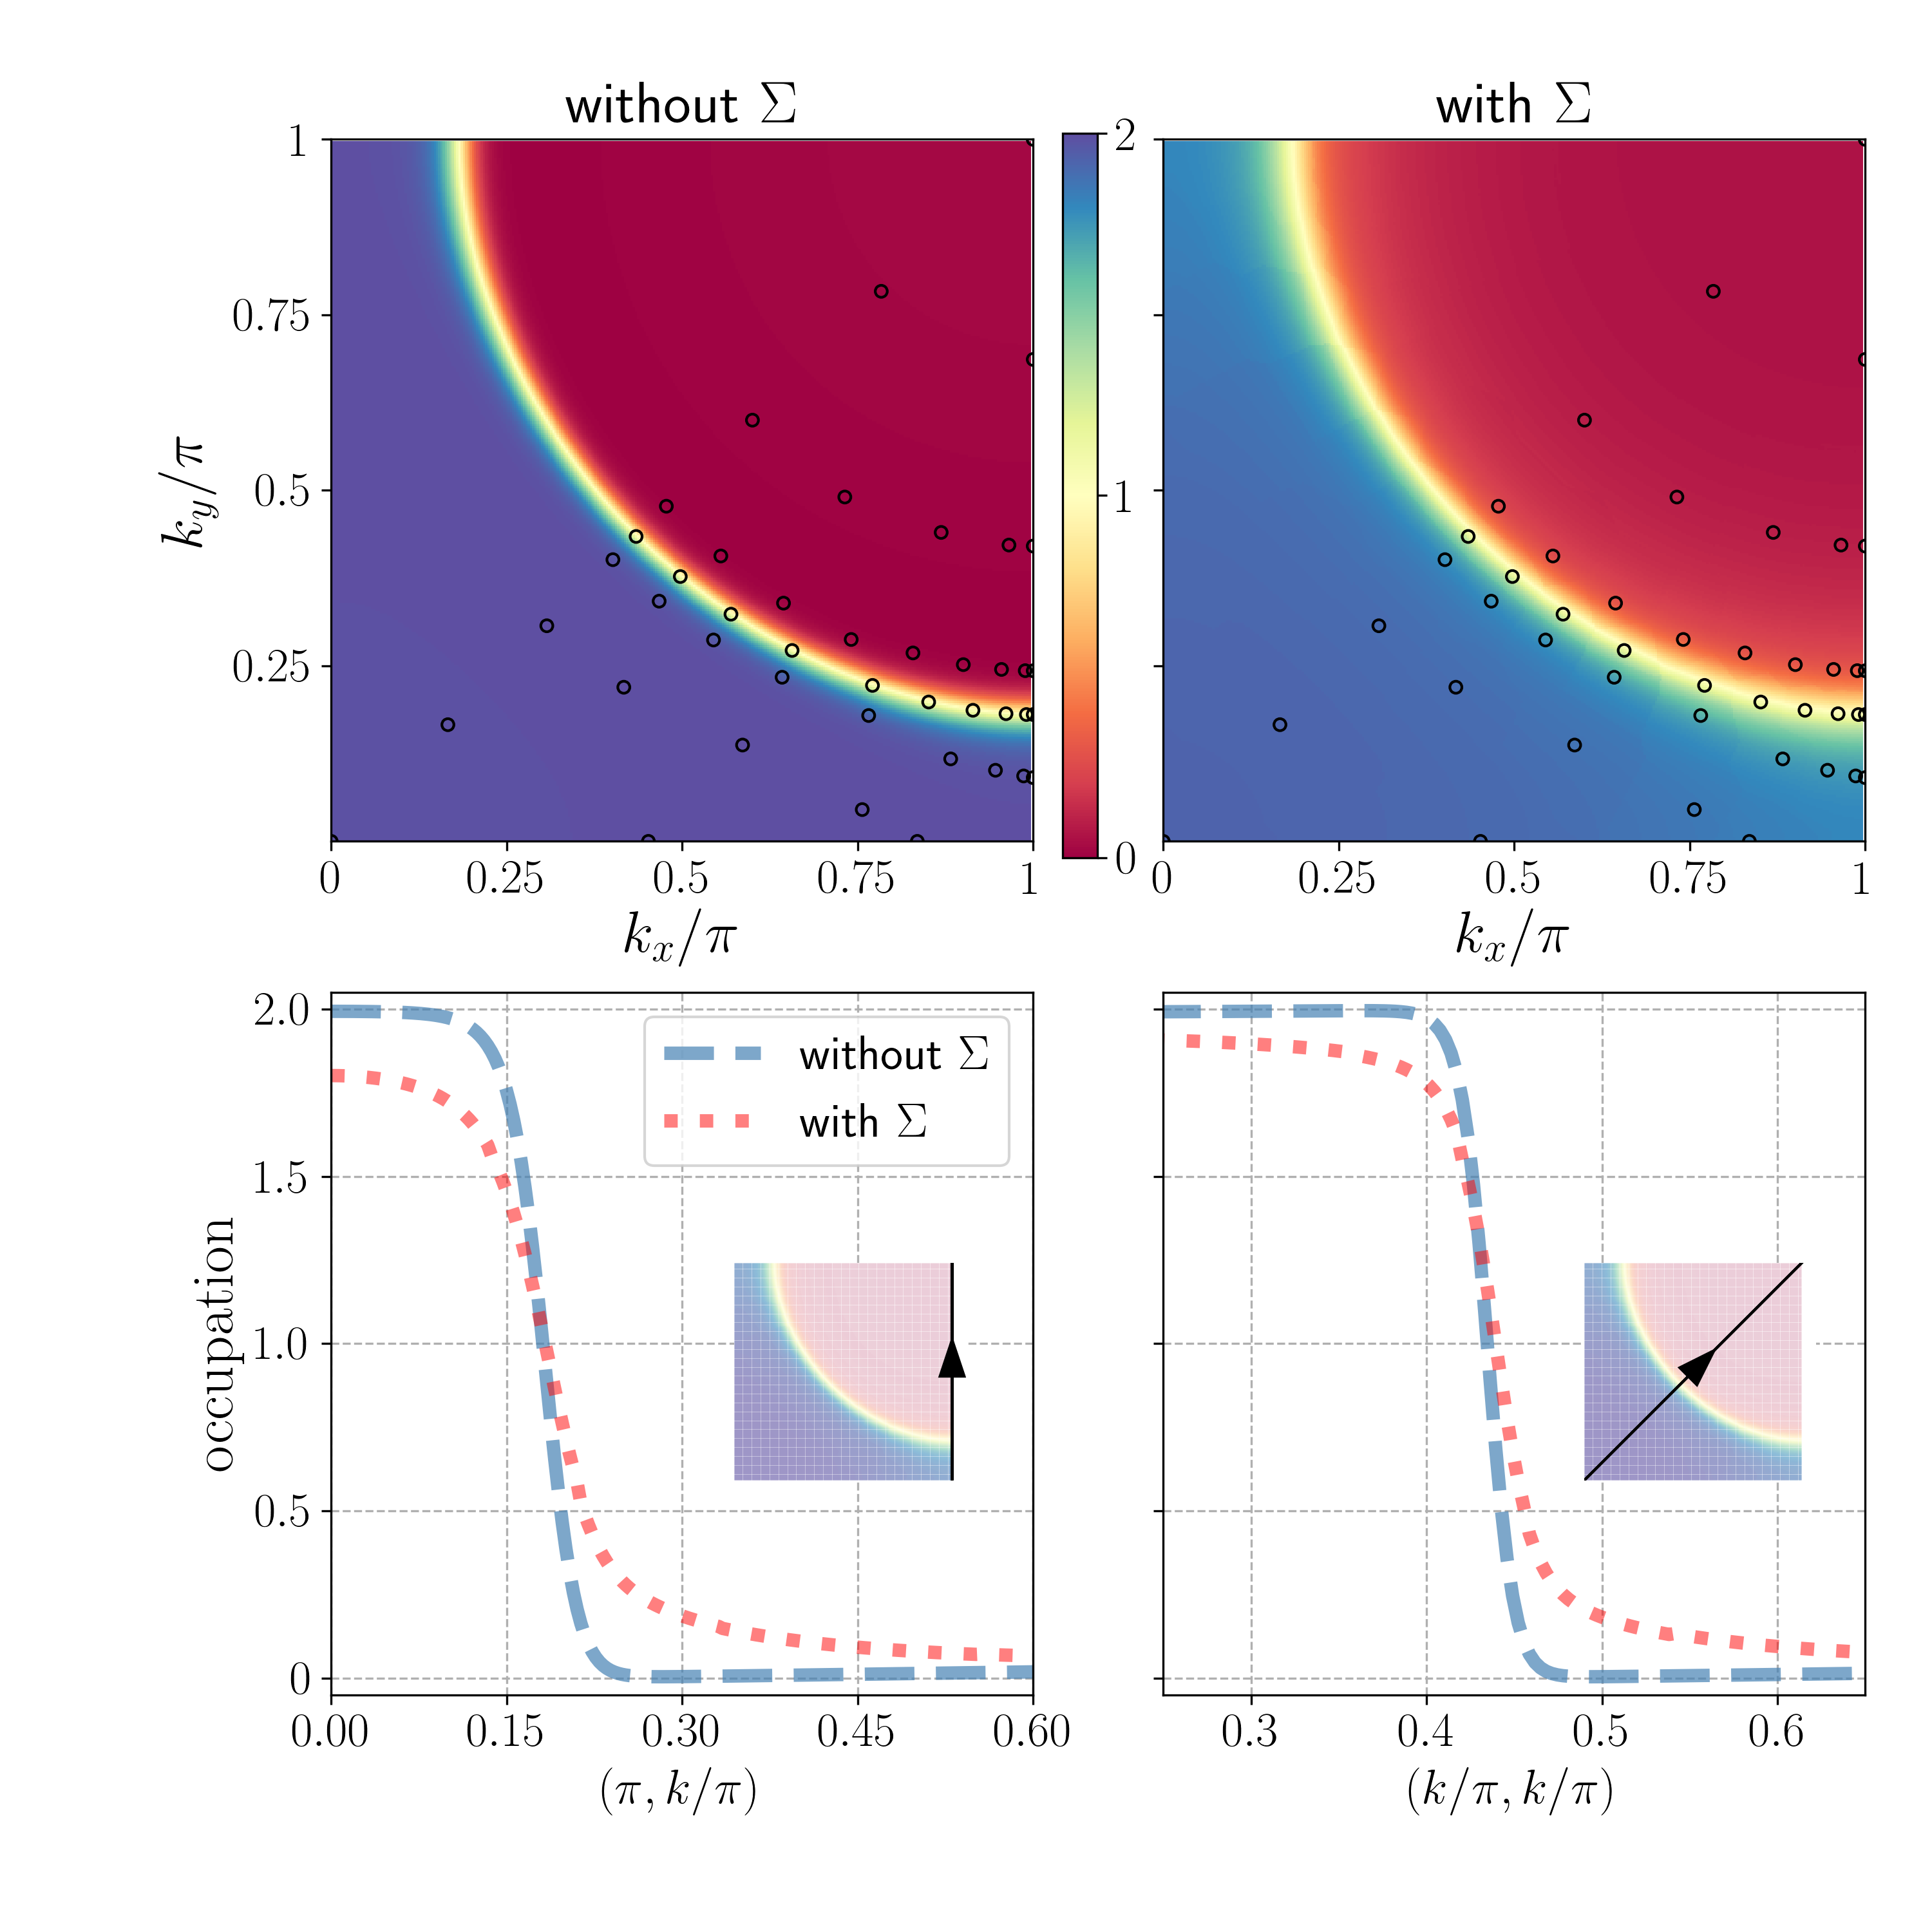
\includegraphics[width=0.5\textwidth]{images/occupations_0975.png}
\caption{Top row: momentum distribution for $t'=-0.32t$, $T=0.08t$ and doping $x=0.025$. Left panel: non-interacting case. Right panel: interacting case for $U=4t$. The black circles mark the points used to patch the self-energy.
Bottom row: cut of the occupation along the Brillouin zone paths reported as arrows in the insets. Blue dashed curves are results for the non-interacting system, while red dotted curves are for $U=4t$. } 
\label{fig:occ975}
\end{figure}

\begin{figure}
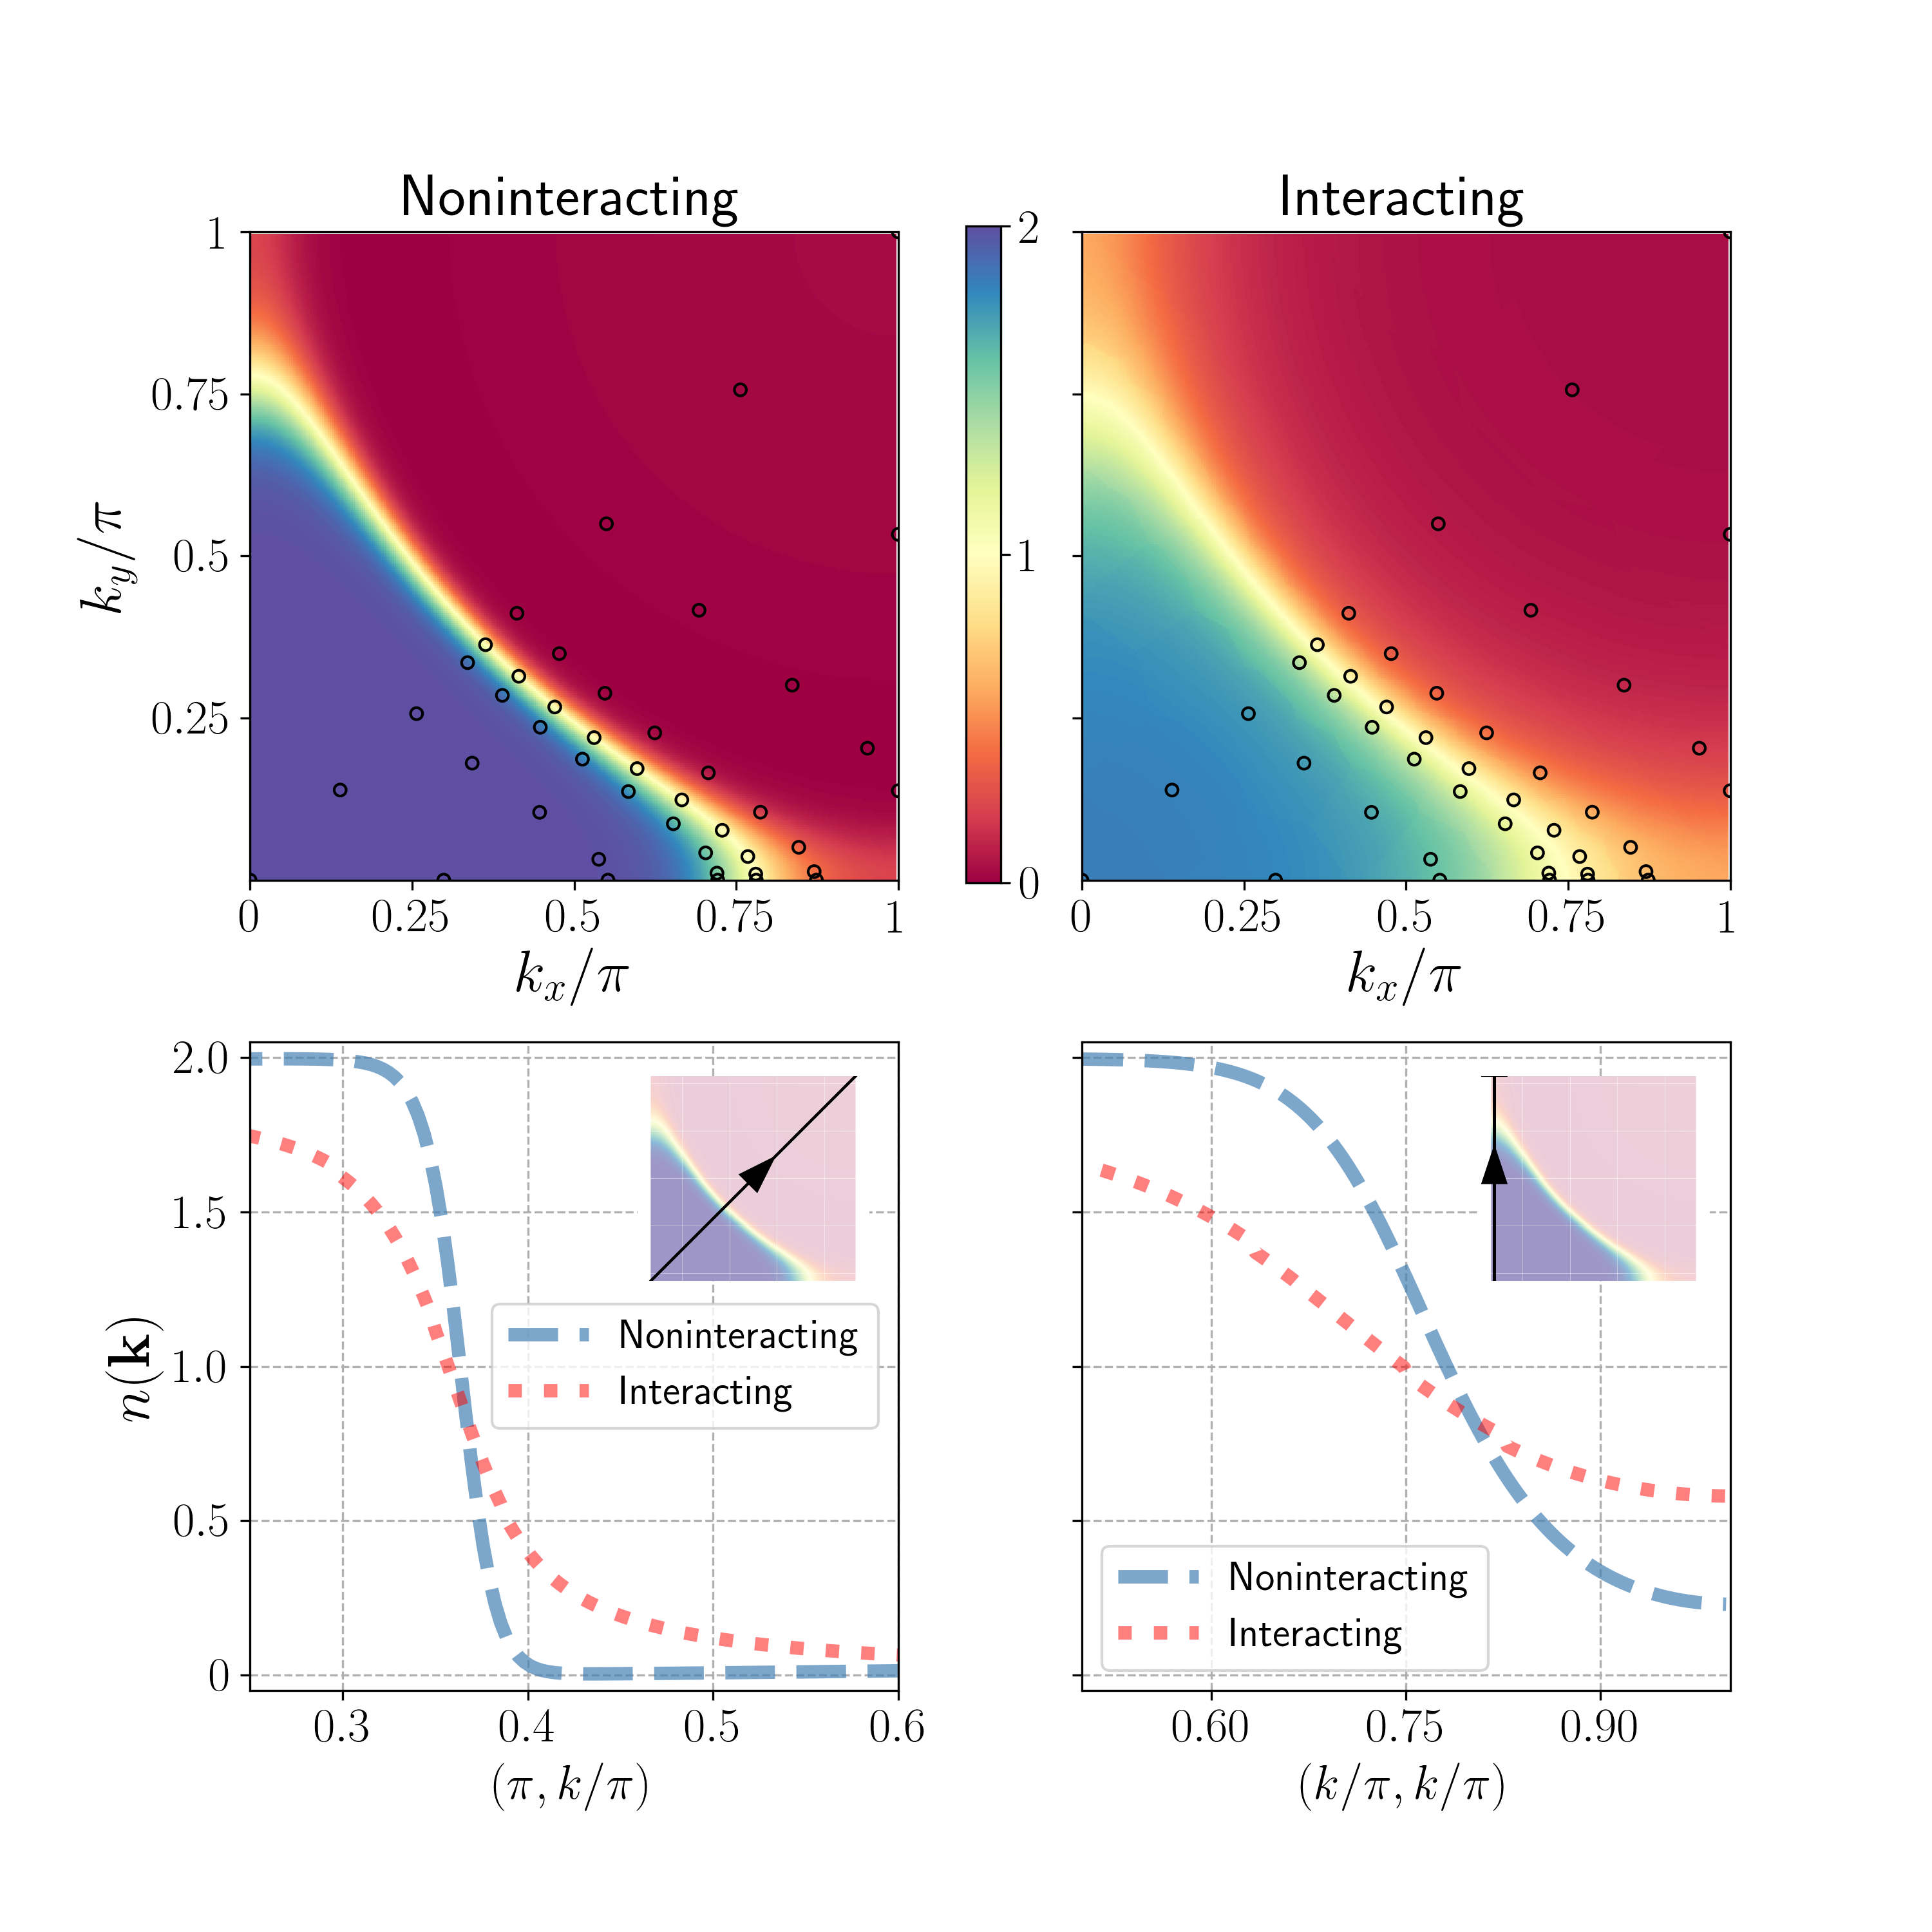
\includegraphics[width=0.5\textwidth]{images/occupations_0600.png}
\caption{Top row: momentum distribution for $t'=-0.32t$, $T=0.08t$ and doping $x=0.4$. Left panel: non-interacting case. Right panel: interacting case for $U=4t$. The black circles mark the points used to patch the self-energy.
Bottom row: cut of the occupation along the Brillouin zone paths reported as arrows in the insets. Blue dashed curves are results for the non-interacting system, while red dotted curves are for $U=4t$. }
\label{fig:occ600}
\end{figure}

To better understand these effects we looked for possible changes in the Fermi surface structure, analyzing the momentum distribution
%
\begin{equation}
 n^{\Lambda}(\mathbf{k})  = 2T \sum_{\nu}\frac{e^{i\nu 0^+}}{i\nu-\varepsilon_\bs{k}+\mu^\Lambda-\Lambda\Sigma^\Lambda(\bs{k},\nu)}.
 \label{eq:occ} 
\end{equation}
%
The factor $2$ accounts for the spin degree of freedom. 
In Fig.~\ref{fig:occ975} we show the non-interacting (top left) and interacting (top right) occupation in the first quadrant of the Brillouin zone for doping $x=0.025$.
The latter is computed at the critical scale $\Lambda_c$. 

Comparing the two panels, one does not observe any relevant shift of the Fermi surface position, but the Fermi surface broadening is appreciably larger in the interacting case, due to the self-energy.
Similar results apply for doping $x=0.4$, as one can see from Fig.~\ref{fig:occ600}, where the broadening is more evident.  

\begin{figure}
\hspace*{-1.0cm}
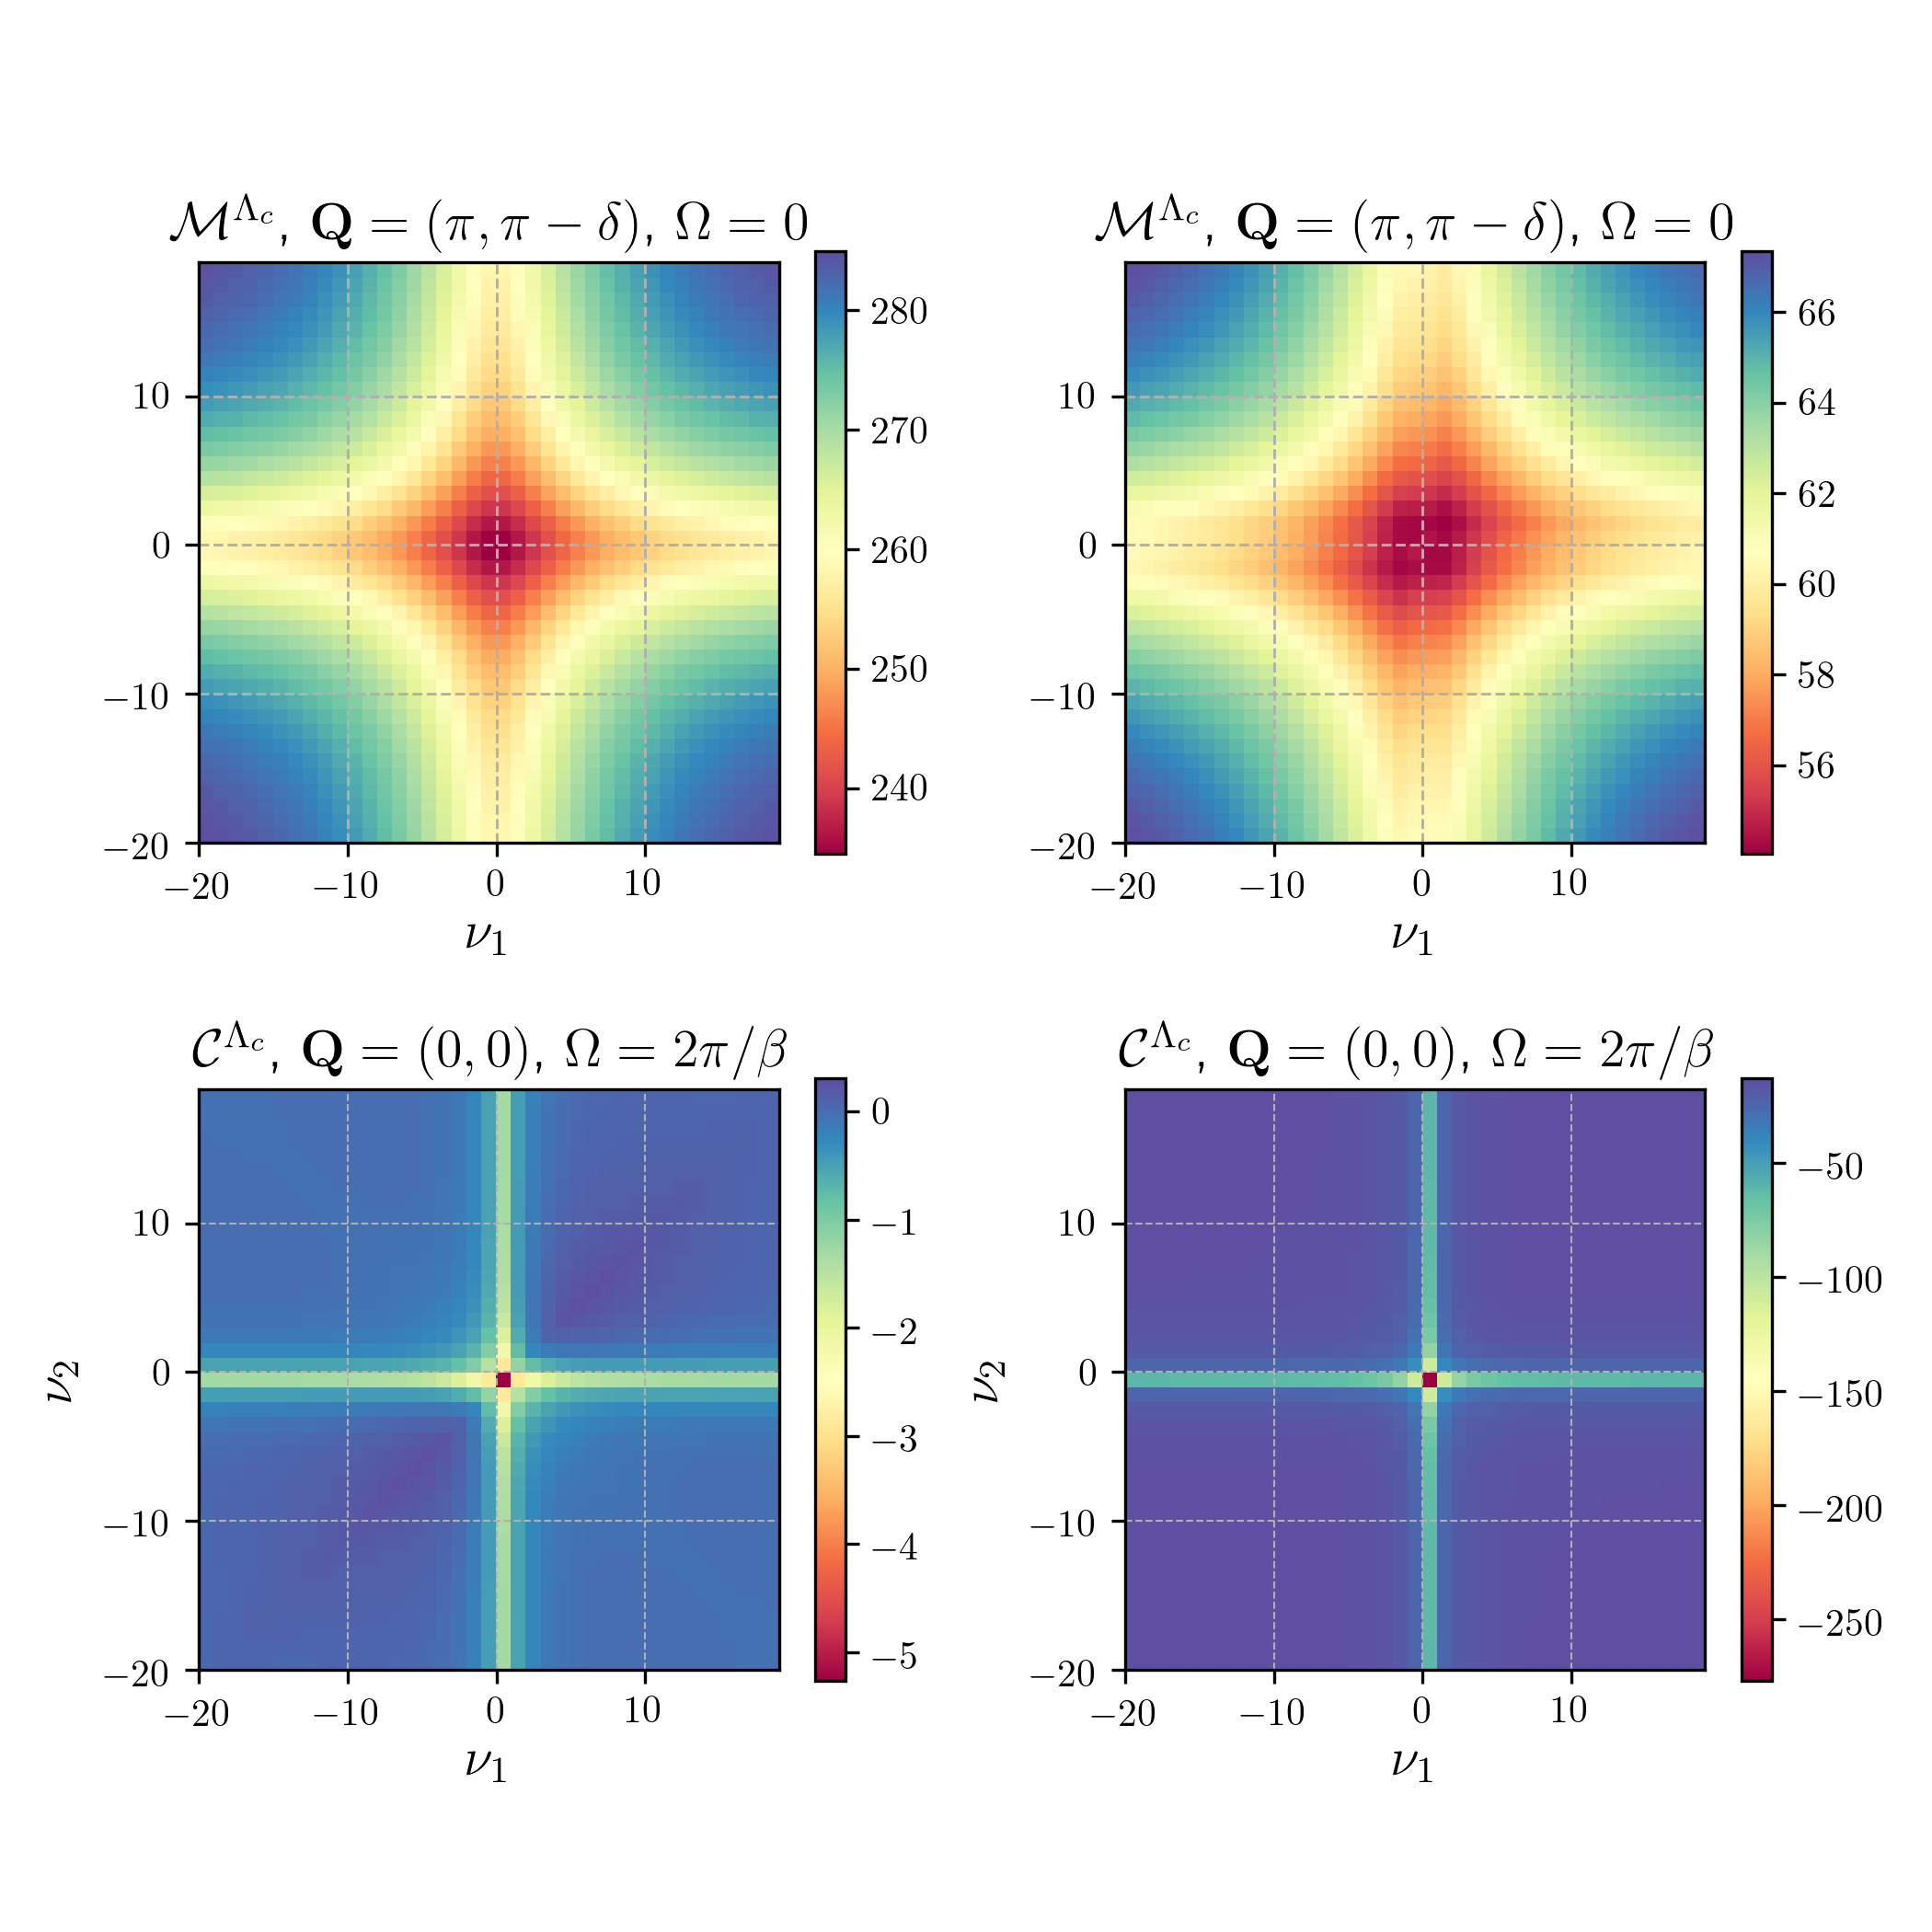
\includegraphics[width=0.52\textwidth]{images/Phi_color_all.png}
\caption{Frequency dependence of the magnetic (top) and charge (bottom) channel for $t'=-0.32$, $U=4t$ and $T=0.08t$.
\emph{Top left}:
Magnetic channel $\mathcal{M}^\Lambda_{\bs{Q},\Omega}(\nu_1,\nu_2)$ with self-energy feedback at the instability vector and for vanishing frequency transfer, for doping $x=0.025$.
\emph{Top right}:
Magnetic channel $\mathcal{M}^\Lambda_{\bs{Q},\Omega}(\nu_1,\nu_2)$ without self-energy feedback at $\mathbf{Q}=(\pi,\pi-\delta)$, $\delta=1.13$ (corresponding to the largest magnetic coupling) and for vanishing frequency transfer, for doping $x=0.4$.
\emph{Bottom left}:
Frequency dependence of the charge channel $\mathcal{C}^\Lambda_{\bs{Q},\Omega}(\nu_1,\nu_2)$ with self-energy feedback at $\mathbf{Q}=(0,0)$ and frequency transfer $\Omega=2\pi T$, for doping $x=0.025$.
\emph{Bottom right}:
Frequency dependence of the charge channel $\mathcal{C}^\Lambda_{\bs{Q},\Omega}(\nu_1,\nu_2)$ without self-energy feedback at $\mathbf{Q}=(0,0)$ and frequency transfer $\Omega=2\pi T$, for doping $x=0.4$.
}  
\label{fig:freqplot} 
\end{figure}

\subsection{Frequency dependence of vertex}

We now discuss the remarkable frequency dependence of the vertex. 
In particular, we will look at the channels that show a divergence, that is, the charge and the magnetic instabilities observed in Fig.~\ref{fig:criscale}, while we refer to the Appendix for the pairing channel.

As mentioned in the previous section the divergences of the charge and magnetic channels are quite different. The charge channel diverges for a finite frequency transfer, and only when we neglect the self-energy feedback. 
Since the dependence on the transfer momentum and frequency $(\bs{Q},\Omega$) has already been discussed in Ref~\onlinecite{Husemann2012}, we focus on the dependence on the fermionic frequencies. Therefore we present various color plots for fixed  $(\mathbf{Q},\Omega)$, showing the dependence on $\nu_1$ and $\nu_2$. 
 
In the top left panel of Fig.~\ref{fig:freqplot} we show the magnetic channel $\mathcal{M}^{\Lambda_c}_{\mathbf{Q},\Omega}(\nu_1,\nu_2)$ in the small doping region, where antiferromagnetism is the leading instability. 
The results shown have been calculated with self-energy feedback, but the frequency structures we discuss do not depend strongly on the presence of the self-energy. 
For clarity we restrict the plots to the first $20$ positive and negative Matsubara frequencies, larger frequencies can be deduced by the asymptotic behavior.\cite{Wentzell2016a}
When only one channel in Eq.~(\ref{eq:vertflow}) is taken into account, the fRG equations are equivalent to the RPA . 
The magnetic channel calculated with RPA would depend only on the frequency and momentum transfer, not on $\nu_1$ and $\nu_2$.
Hence any variation in the frequency structure has to be ascribed to the presence of the other channels in the fRG.
The channel competition suppresses the magnetic channel: the largest value of $\mathcal{M}$ is reduced compared to the RPA, and the frequency dependent structure at the center is further reduced compared to the asymptotic values. 

In the bottom left panel of Fig.~\ref{fig:freqplot} we show the frequency dependence of the charge channel $\mathcal{C}^{\Lambda_c}_{\bs{Q},\Omega}(\nu_1,\nu_2)$ for a finite frequency transfer $\Omega=2\pi/\beta$, related to the charge instability discussed in Ref.~\onlinecite{Husemann2009} and above. 
The frequency structure is completely different from the magnetic channel. 
The charge channel assumes negative values, and the maximum is for frequencies $\nu_1 = \pi T$ and $\nu_2=-\pi T$. 
This structure cannot be explained in terms of standard ladder diagrams. It might be related to the behavior of the retarded interaction described in Ref.~\onlinecite{Stepanov2016}.

In the two right panels of Fig.~\ref{fig:freqplot} we show the same quantities but for $x=0.4$ and without self-energy feedback. In this case, the localized peak in the charge channel is the leading interaction. The position and shape of the frequency structures are similar to the one described above.

\begin{figure*}
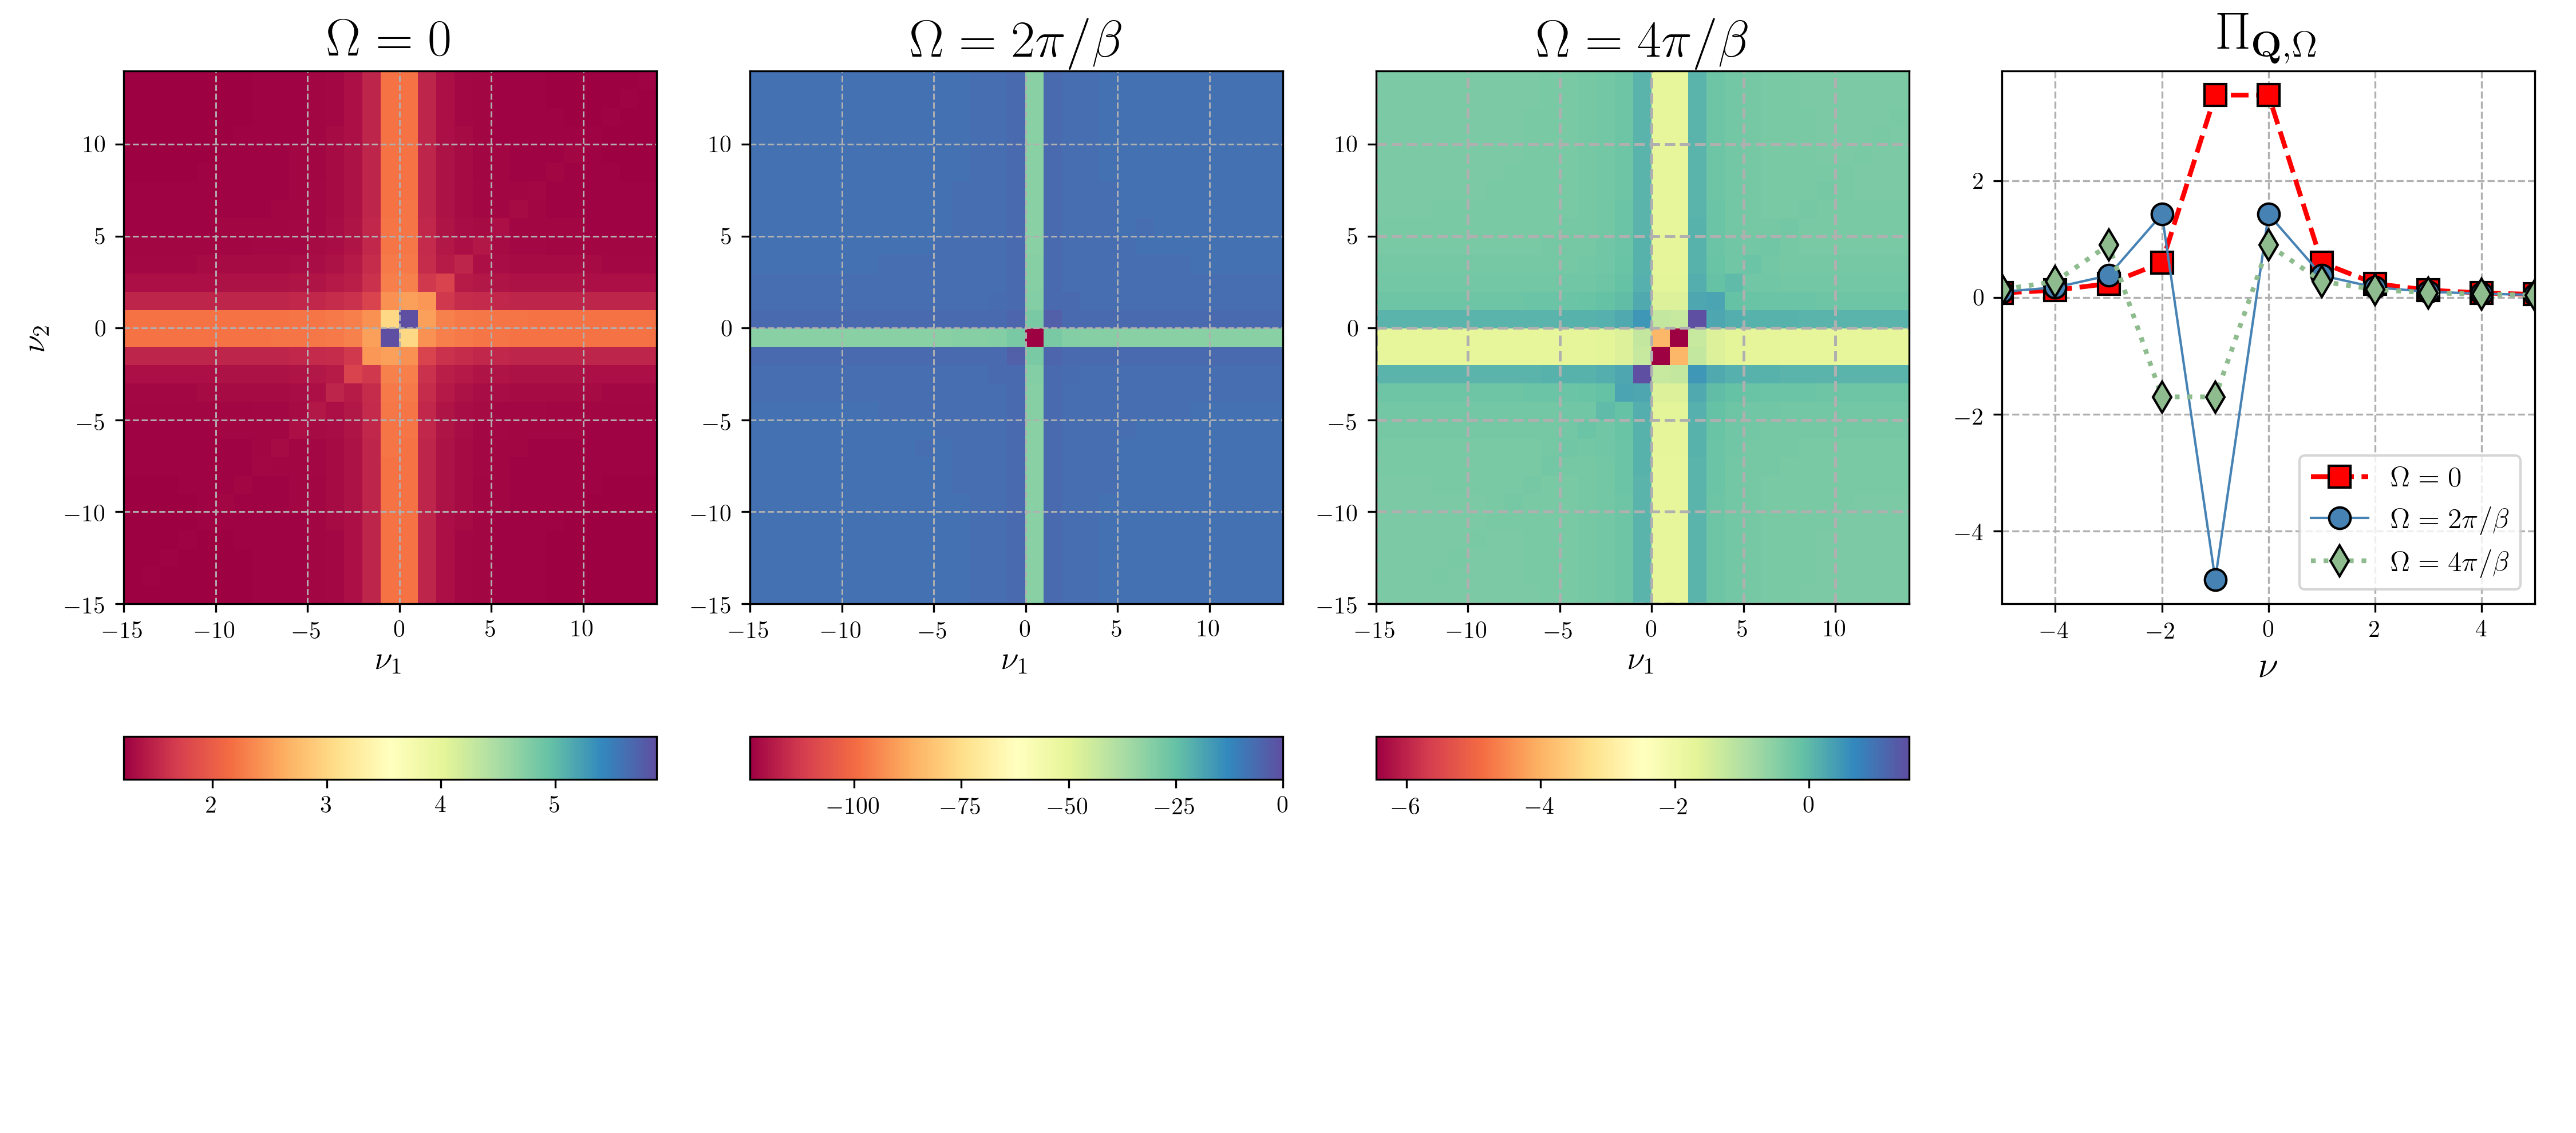
\includegraphics[width=\textwidth]{images/PL_all.png}
\vspace*{-2.0cm}
\caption{In the first three panels from the left, the charge channel $\mathcal{C}_{\bs{Q}=(0,0),\Omega}(\nu_1,\nu_2-\Omega)$ computed from Eq.~(\ref{pl:charge}) is shown as a function of $\nu_1$ and $\nu_2$ for transfer frequencies $\Omega=0$, $\Omega=2\pi T$ and $\Omega=4\pi T$, respectively. In the right panel, the bubble $\Pi_{\bs{Q}=(0,0),\Omega}(\nu)$ is shown as a function of $\nu$ for $\Omega=0$, $\Omega=2\pi T$ and $\Omega=4\pi T$. The model parameters are $t'=-0.32$ and $U=4$, the doping $x=0.375$, and the temperature $T=t$.} 
\label{fig:perpladder}
\end{figure*}

\subsection{Origin of charge singularity} 

To gain insight in the origin of the singular frequency structures observed in the charge channel, we identify a simple set of diagrams reproducing the same features.   
The main idea is that the magnetic channel, which is generated first, is responsible for the singular structure in the charge channel. 

To check this qualitatively, we first compute an effective interaction by means of an RPA in the magnetic channel, and then insert this effective magnetic interaction into a subsequent RPA equation for the charge channel. 
Of course one does not expect quantitative agreement with the fRG, since we overestimate both interactions, but the approximation is sufficient to reproduce and explain the qualitative features we are interested in.  
  
We start by introducing an effective interaction that includes the magnetic fluctuations as computed by RPA \cite{Rohringer2012} in the particle-hole crossed channel:
\begin{equation}
 U^{\mathrm{eff}}_{\bs{Q},\Omega} = \frac{U}{1 - U \Pi_{\bs{Q},\Omega}}.
\label{pl:ueff}
\end{equation}
Since the bare interaction $U$ is local, $U^{\mathrm{eff}}$ depends only on the transfer momentum $\bs{Q}$ and frequency $\Omega$ of the particle-hole bubble
\begin{equation}
 \Pi_{\bs{Q},\Omega} =
 - T \sum_{\nu} \int_{\bs{p}} G_0(\bs{p},\nu) G_0(\bs{p}+\bs{Q},\nu+\Omega).
\end{equation}
The magnetic effective interaction in Eq.~(\ref{pl:ueff}) will be now used to compute the RPA equation for the charge channel. Adopting the simplified momentum dependences of the effective interactions used in the fRG calculation, only the momentum integrated, that is, local part of the magnetic interaction
$U^{\mathrm{eff}}_{\Omega} = \int_{\bs{Q}} U^{\mathrm{eff}}_{\bs{Q},\Omega}$
contributes to the charge channel. We thus obtain
\begin{equation}
\mathcal{C}_{\bs{Q},\Omega} (\nu_1,\nu_3) = U_{\mathrm{eff},\nu_1-\nu_3} \left[ \delta_{\nu_1,\nu_3} + U^{\mathrm{eff}}_{\nu_1-\nu_3} \Pi_{\bs{Q},\Omega}(\nu_1) \right]^{-1} ,
\label{pl:charge}
\end{equation}
where
\begin{equation}
 \Pi_{\bs{Q},\Omega}(\nu) =
 - \int_{\bs{p}} G_0(\bs{p},\nu) G_0(\bs{p}+\bs{Q},\nu+\Omega) .
\end{equation}
Here the charge channel is expressed in terms of $\nu_1$ and $\nu_3=\nu_2-\Omega$ rather than in terms of $\nu_1$ and $\nu_2$. Note that the fermion frequencies $\nu$ are not summed in $\Pi_{\bs{Q},\Omega}(\nu)$.
Eq.~(\ref{pl:charge}) is nothing more than an RPA equation with a frequency dependent interaction in the particle-hole channel.\cite{Rohringer2012} $U^{\mathrm{eff}}$ depends on $\nu_1-\nu_3$ due to the frequency exchange from particle-hole crossed to particle-hole notation.
We note that, in the case of a frequency independent effective interaction $U_{\mathrm{eff}}$, Eq.~(\ref{pl:charge}) becomes $\nu_1$ and $\nu_3$ independent 
and only the summed bubble $\Pi_{\bs{Q},\Omega}$ appears.
The frequency dependence of $U_{\mathrm{eff}}$ qualitatively affects the results. 

In Fig.~\ref{fig:perpladder}, we show the charge channel as computed from Eq.~(\ref{pl:charge}) for $\bs{Q}=(0,0)$  and different $\Omega$ as a function of $\nu_1$ and $\nu_2$, for $T=t$ and $x=0.375$.
We have to choose such a high temperature to stay in a stable paramagnetic phase, due to the above-mentioned overestimation of the fluctuations within the RPA. In the more accurate fRG calculation the magnetic instability occurs at lower temperatures.
The frequency structure in Fig.~\ref{fig:perpladder} for $\Omega=2\pi T$ is very similar to the one shown in Fig.~\ref{fig:freqplot}. 
The simple diagrams considered here reproduce the position of the main structures, as well as the correct sign of the charge channel. 
This is true also for the other bosonic Matsubara frequency shown here, for which we do not report the fRG results. 
Furthermore, upon lowering the temperature the charge channel diverges also for other finite bosonic Matsubara frequencies, while it does not diverge for $\Omega=0$.
From this we conclude that the diagrams described here are responsible for the frequency structure of the charge channel observed in the fRG. 

To understand why the divergence appears for a finite frequency $\Omega$, we notice that in Eq.(\ref{pl:charge}) the $\Omega$ dependence 
appears only through the bubble $\Pi_{\bs{Q},\Omega}(\nu)$. The frequency summed particle-hole bubble obeys the following relation:  
\begin{equation}
 \Pi_{\bs{Q}\rightarrow(0,0),\Omega} = \frac{1}{\beta} \sum_{\nu}
 \Pi_{\bs{Q}\rightarrow(0,0),\Omega}(\nu) = C \delta_{\Omega,0},
\label{pl:sumrule}
\end{equation}
where $C$ is a constant that, at low temperature, approaches the density of states at the Fermi level.
In the rightmost panel of Fig.~\ref{fig:perpladder}, we show the bubble $\Pi_{\bs{Q}=(0,0),\Omega}(\nu)$ as a function of $\nu$ for different values of $\Omega$.
We note that it has a large negative peak for $\Omega=2\pi T$.
This is due to the property (\ref{pl:sumrule}): the summed 
bubble must vanish for $\Omega \neq 0$, hence a large negative value is needed to cancel the positive contributions at large frequency. 
%An argument based on the discontinuity of the bubble, Eq.~(\ref{pl:sumrule}) is also mentioned in Ref. \onlinecite{Stepanov2016}, to justify a possibly related non monotonic behavior of the retarded interaction .
We have thus identified the origin of the frequency structure observed in the charge channel, which seems to be quite general and arises from simple diagrams. 

Including the self-energy in the calculation of the bubble,   Eq.~(\ref{pl:sumrule}) does not evaluate to a $\delta$-function anymore, and the difference between the summed bubble at vanishing frequency and for frequency $2\pi T$ is diminished. 
This is probably the reason why the inclusion of the self-energy feedback prevents the unphysical divergence of the charge channel.     

%All these considerations suggest that the divergence of the charge channel is rather an artefact of fRG without self-energy, arising from a lack of consistence between the vertex and the Green's function in the flow equations. 
%In the next section we further substanciate this conclusion, by explaining the mathematical origin of the feature. 
%The self-energy has qualitative and quantitive effects on the flow equations: quantitively

\subsection{Self energy}

We now discuss the frequency and momentum dependence of the self energy. 
In Fig.~\ref{fig:selffermi0975}  we show the frequency dependence of the imaginary part of the self-energy at $T=0.08t$ and low doping $x=0.025$. 
The spread between the maximal and minimal self-energy at each frequency is rather small, indicating that the self-energy did not develop a large momentum dependence even when the flow parameter reached the critical scale. 
For all momenta, $|\mathrm{Im}\Sigma(\bs{k},\nu)|$ decreases as a function of decreasing frequency, as in a Fermi liquid. 
One would generally expect the antinodal region to be more affected by correlation effects. However, there is only a slight increase of $|\mathrm{Im}\Sigma(\bs{k},\nu)|$ in this region. At the temperature we are considering, we do not observe a tendency towards the opening of a momentum selective gap. 

In Fig.~\ref{fig:selffermi0600} we show the imaginary part of the self-energy for a larger doping $x=0.4$. As in the previous case, we do not see much momentum differentiation.

The self-energy enters directly in the calculation of the momentum distribution through the Green's function, already discussed above, and shown in Figs.~\ref{fig:occ975} and~\ref{fig:occ600}.
In the bottom panels of these figures, we show how the momentum distribution evolves along two different cuts in the Brillouin zone, crossing the \textit{nodal} and \textit{antinodal} regions, respectively.
The drop in the momentum distribution is sharper along the diagonal, and the self-energy effects are stronger along the antinodal cut.
For doping $x=0.4$ the broadening of the Fermi surface, already larger at the non interacting level, is further enhanced by the self-energy.

To study further the difference between nodal and antinodal regions in the iAF case, we studied the quasiparticle weight\cite{Abrikosov1963,Metzner2012} $\mathcal{Z}_{\bs{k}}$, and the decay rate $\gamma_{\bs{k}}$.
Instead of relying on analytical continuation, we have extracted the parameters directly from the imaginary axis data.
To do so we have fitted the first few frequencies of the imaginary part of the self-energy with a polynomial of degree $l$: $\mathrm{Im}\Sigma(\bs{k},i\nu)\approx a_0(\bs{k})+a_1(\bs{k})\nu+...+a_l(\bs{k})\nu^l$ and we identified $\gamma_{\mathbf{k}}=a_0(\bs{k})$ and $\mathcal{Z}_{\bs{k}}= \frac{1}{1-a_1(\bs{k})}$.
The procedure only works if the temperature is small enough, and if the frequencies used for the fitting are not too high. We checked that the results were stable by changing the number of frequencies and the order of the polynomial used for the fit. 
In Fig.~\ref{fig:zetaandgamma} we plot $\mathcal{Z}_{\bs{k}}$ and $\gamma_{\bs{k}}$ against the angle $\theta$ along the Fermi surface, $\theta=0$ corresponding to the antinodal point and $\theta=\pi/4$ to the nodal one. 
The variation of the quasiparticle weight along the Fermi surface is extremely small with $\mathcal{Z}$ assuming values between $0.754$ and $0.760$. 
On the other hand, the relative variation of the decay rate $\gamma$ along the Fermi surface is sizable, varying from $\gamma\approx 0.056t$ and $\gamma \approx 0.082t$. These values are comparable with the temperature $T=0.08t$. 
We conclude that at the critical scale, the system still has coherent quasiparticles along the Fermi surface, with a higher decay rate in the antinodal region. This is consistent with the observations of Ref.~\cite{Rohe2005}, where non-Fermi liquid behavior of the self-energy was observed only very close to the critical temperature and in the immediate vicinity of the hot spots. \emph{Honerkamp}  
\begin{figure}
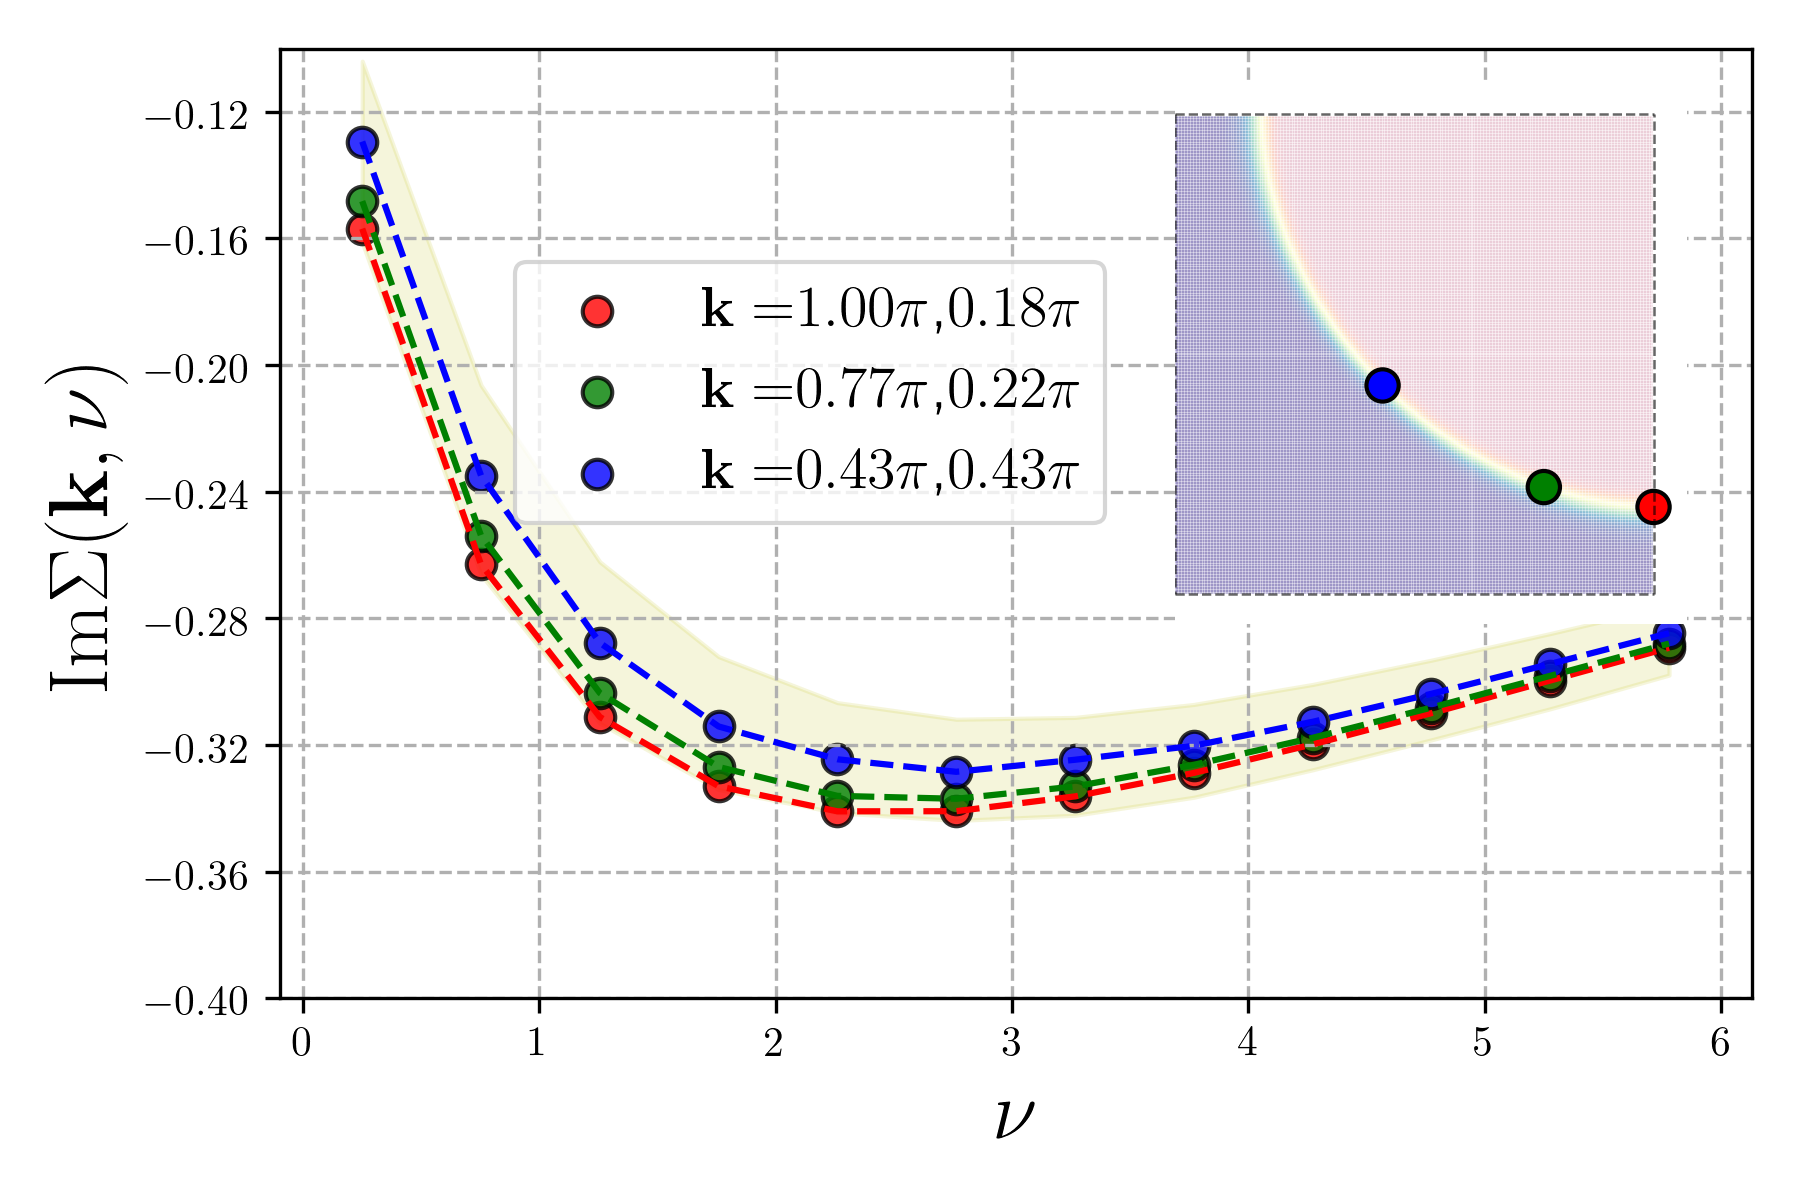
\includegraphics[width=0.50\textwidth]{images/Self_Im_occ0975.png}
\caption{Self-energy as a function of frequency for $U=4t$, $t'=-0.32t$ and low doping $x=0.025$ at a temperature $T=0.08t$.
The location of the $\mathbf{k}$-point in the Brillouin zone is color coded in the inset. The position of all the patching points taken into account for the self-energy is shown as black circles in the top row of Figs.~\ref{fig:occ975} and \ref{fig:occ600}, and does not change during the flow.
The shaded area highlights the region between the maximal and minimal value of the self-energy for each frequency. }
\label{fig:selffermi0975}
\end{figure}

\begin{figure}
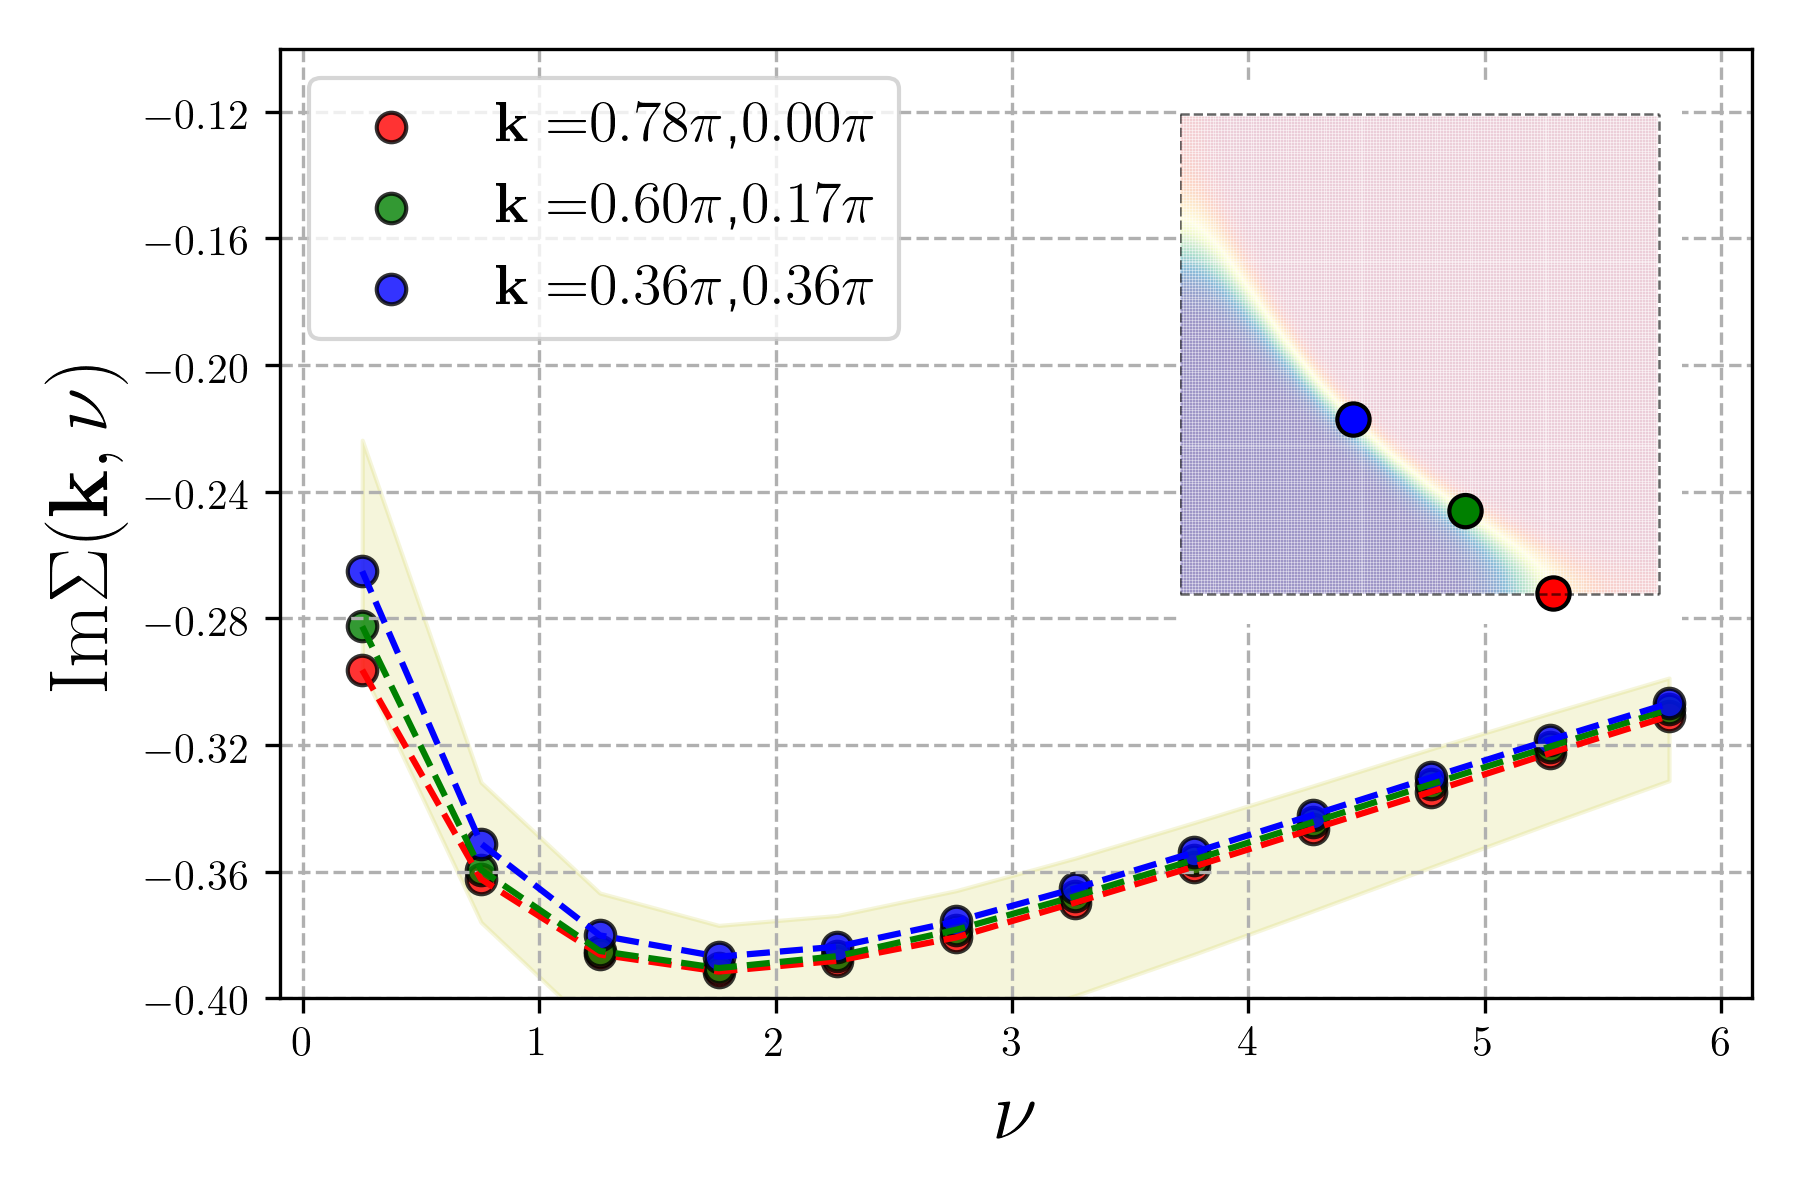
\includegraphics[width=0.50\textwidth]{images/Self_Im_occ0600.png}
\caption{Self-energy as a function of frequency for $U=4t$, $t'=-0.32t$ and high doping $x=0.4$ at a temperature $T=0.08$.
The location of the $\mathbf{k}$-point in the Brillouin zone is color coded in the inset. The position of all the patching points taken into account for the self-energy is shown as black circles in the top row of Figs.~\ref{fig:occ975} and ~\ref{fig:occ600}, and does not change during the flow.
The shaded area is the region between the maximal and minimal value of the self-energy for each frequency.}
\label{fig:selffermi0600}
\end{figure}

\begin{figure}
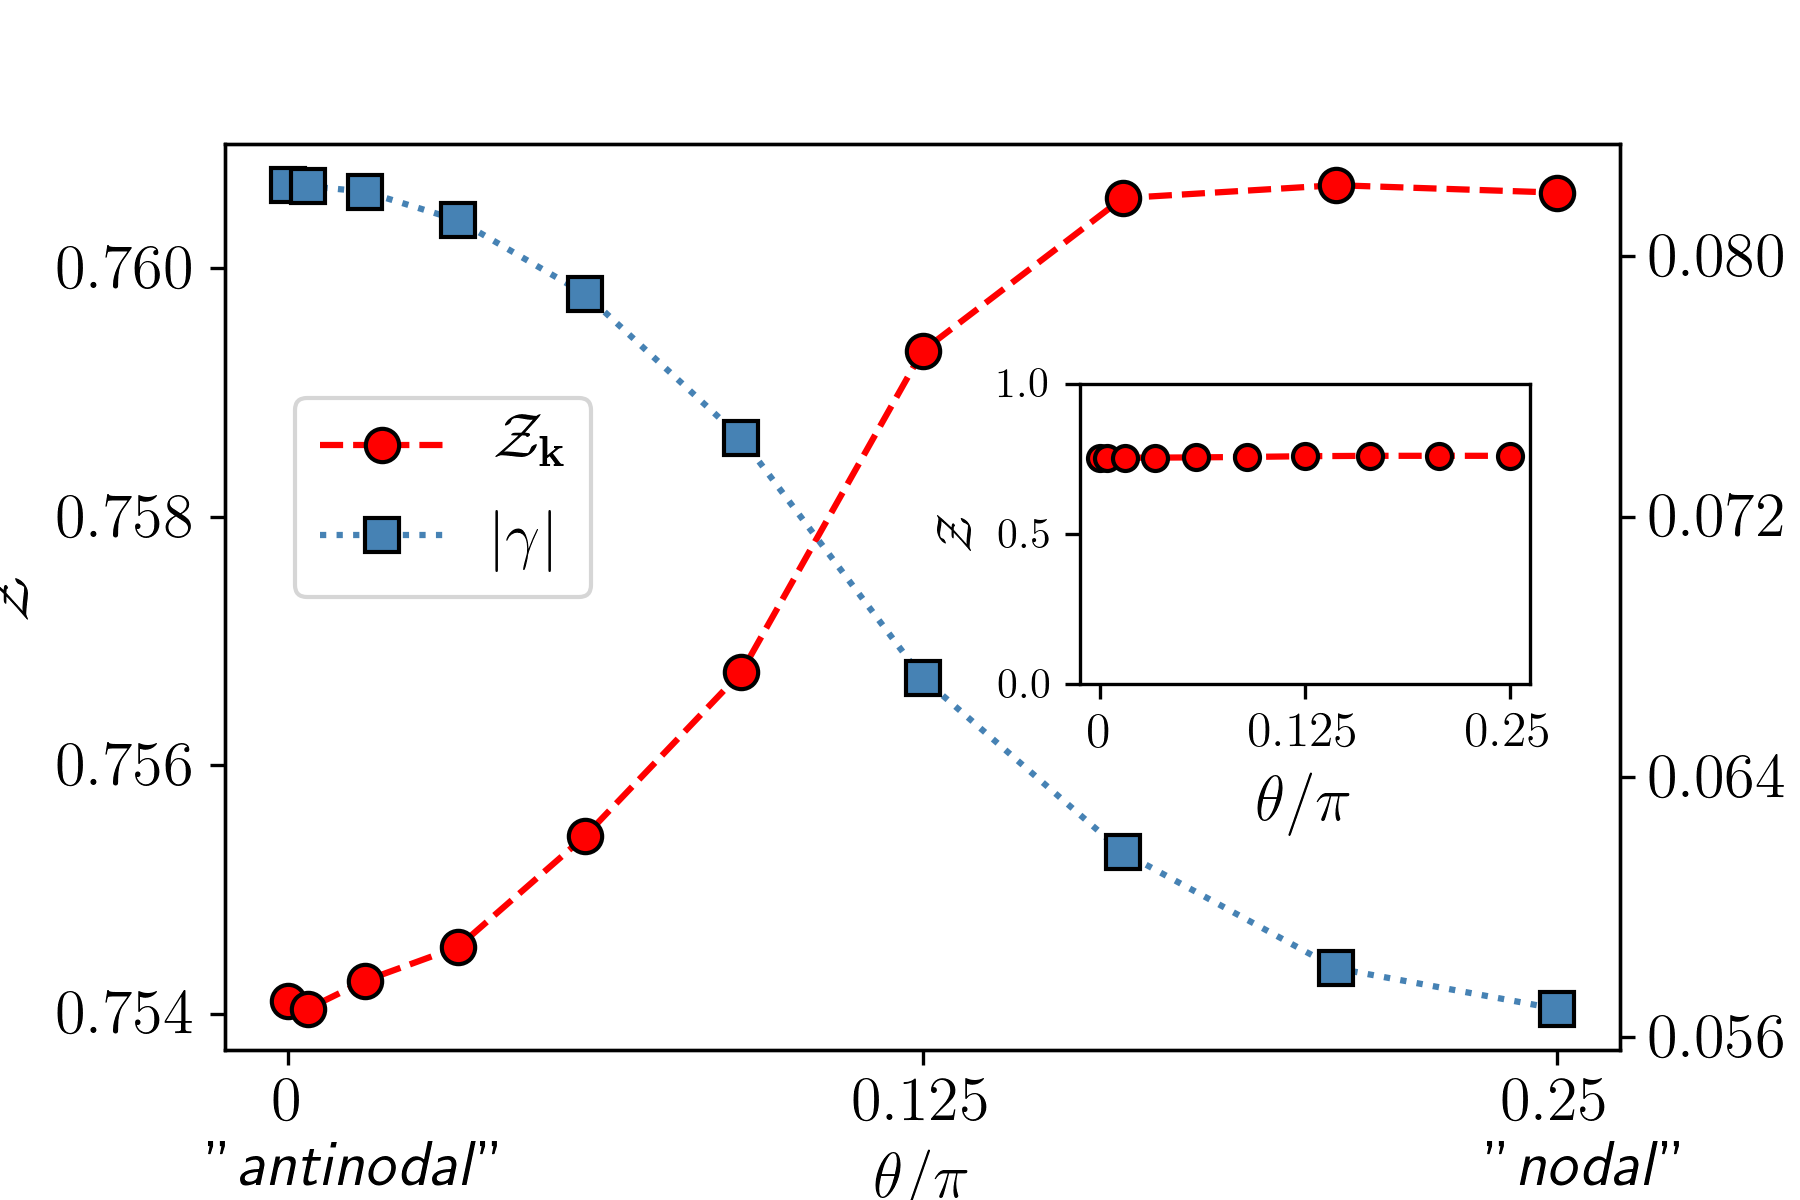
\includegraphics[width=0.5\textwidth]{images/z_and_gamma975.png}
\caption{Quasiparticle weight $\mathcal{Z}_{\bs{k} }$ and decay rate $\gamma_{\bf{k}}$ as function of the angle $\theta$ for the same parameters as in Fig.~???. 
The values on the left axis refer to the quasiparticle weight, the values on the right axis refer to the decay rate.}
\label{fig:zetaandgamma}
\end{figure}
